\documentclass[11pt, rgb]{scrreprt}
\usepackage{themeKonstanzDBIS} % Muss immer verwendet werden (Standardpaket)

\usepackage{algorithm}
\usepackage{algorithmicx}
\usepackage{algpseudocode}
\usepackage{mathtools}  % amsmath with extensions
\usepackage{amsmath} 
\usepackage{amsfonts}  % (otherwise \mathbb does nothing)
\usepackage{amssymb}  % (otherwise \mathbb does nothing)
\usepackage{nameref}
\usepackage{pgfplots}
\usepackage[normalem]{ulem}
\usepackage{array,booktabs,ragged2e}
\usepackage{pgf-umlcd}
\usepackage{wrapfig}
\usepackage{float}
\usepackage{eurosym}





\format{a4}

% Thesis information        %
%\date{\today}
\year{2023}
\author{Marius Hahn}
\title{Master Thesis}
\subtitle{thesis}
\unisection{Faculty of Sciences}
\department{Department of Computer and Information Science}
\supervisorOne{Prof. Dr. Theodoros Chondrogiannis}
\supervisorTwo{Prof. Dr. Sabine Storandt}

\headFoot{14}

%%%%%%%%%%%%%%%%%%%%%%%%%%%%%%%%%%%%%%%%%%%%%%%%%%%%%%%%%
% Begin vom Dokument                                    %
%%%%%%%%%%%%%%%%%%%%%%%%%%%%%%%%%%%%%%%%%%%%%%%%%%%%%%%%%

\begin{document}

% Thesis Title
\thesistitlepage[language=english]{Query Processing on Dynamic Networks with Customizable Contraction Hierarchies on Neo4j}

\chapter*{Abstract}

% Table of Contents           
\tableofcontents

%Use only if thesis is over 100 pages.
% List of figures
%\listoffigures
%\addcontentsline{toc}{chapter}{List of Figures}

%Use only if thesis is over 100 pages.
% List of tables
%\listoftables
%\addcontentsline{toc}{chapter}{List of Tables}

% For chapters and sections use  
%    \chapter{...}
%    \section{...}
%    \subsection{...}
%    \subsubsection{...}
%

\rmfamily 
\normalsize

\chapter{Introduction}

Most applications which handle data have to store these eventually.
Simple files do not offer enough semantic structure.
Therefore databases have been developed to not only store but query and aggregate data effectively and efficiently.
Relational databases that store data in tables have become the unspoken industry standard in the last decades. 
However there are domains that do not naturally fit into tables and one will need a lot of restructuring to make them fit.
As a result, there have been efforts to create databases that use other abstractions to store data, like the graph database Neo4j.

\section{Background and Motivation}

In a relational database the data is organized in tables.
Tables have rows and theses rows can be connected to other rows of the same or a different table using joins on matching cells, usually primary- foreign key relationships.
To retrieve information that is stored in two table rows one has to scan both an join them on the desired key property.
Depending on the size of the tables and the number of joins which have to be done to retrieve the desired information, such queries can be very expensive.
\\
In contrast to relational databases, graph databases treat relationships as first-class citizen.
This means a relationship that connects nodes is an entity just as the nodes it connects themselves.
As in a graph database, a node has a pointer to its relationship and a relationship has a pointer to its nodes, there is no table scan needed to retrieve connected data, which can make these queries very performant.
Such queries are shortest path queries on domains which resembles a graph by their nature, for instance road networks. 

\section{Problem and Objectives}

We focus on these shortest path queries and try to make these even quicker by employing an index call Customization Contraction Hierarchies \cite{CCH}, \textit{CCH}. 
CCH is proven to achieve a tremendous speedup compared to Dijkstra's algorithm in graphs where one can find vertices that are more important than others.
Important in this context means that these vertices belong to many shortest paths.
One example for such a domain are road networks, which we will also use in our test scenarios.

\section{Contribution}

In comparison to many other papers that examine CCH in their specific details we want to examine if we can adopt it to the graph database Neo4j, and still keep its advantages.
Will we be able to store the index in a manner which allows us to keep the performance gain we had achieved before?
Additionally we want to explore how the index behaves after updating multiple edge weights.
Will queries still be as quick as they were before the update?
This is an essential question as data in databases are usually not only stored but also manipulated.
We also want to uncover how big such an index graph will become, as there might be no need to read the index from the disk, because it easily fits in main memory.
\\
Finally we want to keep the integration into Neo4j as small as possible to make it as easy as possible at a later point to port the implementation to other graph databases that might become more relevant in future.

\chapter{Related Work} 

As our research focus is set ti databases, we want to divide this chapter in two main sections \nameref{sec:algorithmic_history} and \nameref{sec:related_work:database}.
\nameref{sec:algorithmic_history} that will give some basic overview what has been published regarding index structures to speed up shortest path queries for graphs.
\nameref{sec:related_work:database} we will try to give an overview of efforts that have been made to make \cite[Customizable Contraction Hierarchies]{CCH} it suitable for graph databases.

\section{Speed Up Dijkstra's algorithm} \label{sec:algorithmic_history}

The basic algorithm to answer shortest path queries is \cite[dijkstra]{Dijkstra_1959}.
It is from 1959 and in the decades after it there have been many approaches to get it quicker.
To name some there is \cite[A*]{A_Star}, which adds a heuristic to each node to help dijkstra to go in the right direct.
Then there is \cite[ALT]{ALT} with stands for \textit{A* + Landmarks + Triangle Inequality}, which is a approach to improve the A* heuristic with landmarks.
Then there is the \cite[Arc Flag]{ARC_FLAG} approach that which is based on the idea that many shortest paths in a graph usually overlap, so we can store them in a compact way.
Later only edges which are flagged true for the target direction will be expanded by dijkstra.
Then there is the \cite[Transit-Node]{Bast_2007} that makes use of the observation that if you want to go far, nodes that are spacial close usually pass by the same node.
One will try to find such nodes and store their connecting shortest paths in a table.
If one looks for the way from one to another node one only starts to local dijkstra for the source and the target side until one finds a transit node.
As the distance between the transit nodes are known, we simply can look up the rest of the path.
Then there is \cite[Contraction Hierarchies]{Geisberger_2012} or CH which is the base for what we will examine further.
As transit nodes, CH goes with the idea that there are nodes that are more important than others, but instead of selecting some important nodes one ranks them all.
CCH, what we will implement for Neo4J, is a fashion of CH that makes it easier to react to changes in the CH index structure.
CH goes back to the diploma thesis of \cite[Geisberger]{Geisberger} in 2008.
As all previous mentioned techniques, CH and CCH especially speed up long distance queries.
\\ 
CH deletes nodes and inserts edges to the graph, so called shortcuts, that preserve the shortest path property in case a node that is deleted resides on a shortest path between remaining ones.
When querying a shortest path, CH uses a modified bidirectional-dijkstra that is restricted to only visit nodes that are of higher importance, called rank, than the its about to expand next.
This method is able to retrieve shortest paths of vertices that have a high spacial distance.
However, it is rather static.
In case a new edge is added or an edge weight is updated, it might be necessary to recontract the whole graph to preserve the shortest path property.
\\
In 2016 \cite[Customization Contraction Hierarchies]{CCH} or CCH was published.
The approach is the same, but in CCH shortcuts are not only added if the contraction violates the shortest path property.
Shortcuts are added if there had been a connection between its neighbors through the just contracted vertex and these neighbors do not own a direct connection through an already existing edge.
The shortcut weights are later on calculated through the lowers triangle.
Additionally \cite[Customization Contraction Hierarchies]{CCH} provides an update approach that only updates,
edges that are affected by a weight change.


\section{Existing shortest path algorithms in Neo4j}

Neo4j contains a implementation of dijkstra, bidirectional dijkstra and an A* implementation out of the box.
They are provided by the traversal API, such that every plugin can use it.
Sadly the only provide a \textit{one to one} dijkstra, which made it useless for our purpose.
Additionally the tests that prove our dijkstra implementation as stated in \ref{sec:dijkstra}, uses the neo4j bidirectional dijkstra and compares the path weights.
By that we also measure the time both need to find the shortest path.
It shows our unidirectional dijkstra is slightly faster than the one of neo4j.
\\
Then there is the neo4j graph data science library  which provides a \textit{one to all} and \textit{one to one} dijkstra implementation.
Additionally it contains also a A* implementation, a \textit{Yen’s Shortest Path} algorithm and a \textit{Delta-Stepping Single-Source Shortest Path} algorithm.
We did't use these neither as it turned out, having our own dijkstra is key to get the implementation we are looking for.

\section{Shortest path query processing with external memory}

Most shortest path external memory approaches have focused on Hub-Labels like "HLDB: location-based services in databases \cite{Abraham_2012}" and "COLD. Revisiting Hub Labels on the database for large-scale graphs \cite{efentakis2015cold}", with a few notable exceptions like "Mobile Route Planning \cite{Sanders}" and "The case against specialized graph analytics engines" \cite{fan2015case}.
Hub-Labels tries to find important vertices that are encoded in many shortest path, so called "hubs". 
After that it precalculates a two hop cover for all vertices in the graph.
For every source target vertex pair $s$, $t$ there must be at least one common hub $\forall s,t \epsilon V \exists h \epsilon H(s) \cap H(t)$ \cite{Abraham_2011} and saves this information to a so called hitting set $H$. 
Each vertex has its own hitting set. 
For query answering on looks in the hitting set of the source and the target vertex. 
There must be at least one common hub.
With adding the distances that are stored in the two hitting sets on gets the distance from $s$ to $t$.
By recursively looking at the neighbors of the target vertex one can finally resolve the original path. 
This method is faster than CH due to \cite{Abraham_2012} but the space consumption is higher as well as the preprocessing time. 
HLDB \cite{Abraham_2012} uses a relational database to store and query the hitting set of vertices.

\section{Contraction Hierarchies in Neo4j}\label{sec:related_work:database}

There is one bachelor thesis by Nicolai D'Effremo \cite[Some text]{DEffremo2019} that has implemented a version on \cite[Contraction Hierarchies]{Geisberger_2012} for Neo4j.
This implementation shows that even for databases CH is an index structure worth pursuing, as there was a tremendous speedup of shortest path queries paired with a reasonable preprocessing time.
\cite{Zickenberg2021} showed in his bachelor thesis that it is even possible to restricted these queries with label constraints.
Although CH and CCH have little difference, sadly we could not use much of the code provided by there works.
It was deeply integrated into the Neo4j-Platform.
Additionally since then two major release updates happened that have breaking changes which make it nearly impossible to reuse any of this code.
\\
Finally there is \cite[Mobile Route Planning]{Sanders} by Peter Sanders, Dominik Schultes, and Christian Vetter.
In this paper it is described how one can efficiently store the a CH index structure on a hard drive.
It states an interesting technique to how store edge that are likely to be read sequentially spatially close on the hard drive which makes read operations that have to be done during query time fast.
The motivation of \cite[Mobile Route Planning]{Sanders} through was slightly different.
They came up with this idea because computation power on mobile devices is limited, so they could precalculate the CH index on a server and then later distribute it to a mobile device.
\\
We will use parts of this idea and partly port it to our database context as we suppose there are many similarities.

\chapter{Preliminary}

As the target platform for this work is the graph database neo4J, we will mostly consider \textit{directed} graphs. From the terminology we always refer \textit{arcs}, which is an directed edge.
In some cases we will refer to \textit{edges}, in these cases the direction doesn't play a role.

\section{Notation and Expressions}
We denote a graph $G(V, A)$ in case me mean an \textit{directed} graph, where $v$ is a vertex contained in the vertices $v \epsilon  V$ and $a$ is an
arc $a \epsilon A$. An arc is uniquely defined by to vertices $v_a$ and $v_b$ such that $v_a \neq v_b$, so there are no loops nor multi edges.
An edge additionally has a weight function $w: A \rightarrow \mathbb{R}_{<0} $ it's weight which must be a positive.
\\
We use $A$ as the arc set and $a$ a single arc which is directed. $a \epsilon A$ can be replace with $e \epsilon E$ which refers to edges that are \textit{undirected}. 
\\
$G$ represents the input graph. The contraction graph $G'(V', A')$ is the graph that will be used at contraction for initially building the CCH index structure. A vertex $v$ in will 
never be really deleted. Instead the rank property $r(v)$ is set to mark this as an already contracted. So $V \equiv V'$ but $A \subseteq A'$ there will be edges add while building
the CCH index. $S = A' \setminus A$ is the shortcut set that is added throughout the contraction. 
\\
$G^*(V^*, A^*)$ is the is the search graph while doing one a shortest path query. Futhermore one query will have two search graphs. $G^*_\uparrow$ representing the upwards search graph
and the $G^*_\downarrow$.
\\
Finally there will be the edge set of edges that are written to the disk. These will $\bigcirc A$ will be separated into to sets $\bigcirc A_\downarrow$ and $\bigcirc A_\uparrow $, too.


\section{Customizable Contraction Hierarchies}\label{sec:Preliminary_CCH}

In this section we will present the basic idea of \cite[Customization Contraction Hierarchies]{CCH} and also work out the main difference between CCH and \cite[Contraction Hierarchies]{Geisberger_2012}.
It is far form being complete, but there will be some easy examples to show the concept. 

\subsection{Contracting and Searching}

\begin{figure}
    \centering
    \begin{tikzpicture}[node distance={15mm}, main/.style = {draw, circle}]

    \node[main] (x11) at (0, 0) {$3$};
    \node[main] (x21) at (1, 0) {$1$};
    \node[main] (x31) at (2, 0) {$5$};
    \node[main] (x41) at (3, 0) {$2$};
    \node[main] (x51) at (4, 0) {$4$};
    
    \draw (x11) -- (x21);
    \draw (x21) -- (x31);
    \draw (x31) -- (x41);
    \draw (x41) -- (x51);
    \draw[dashed, out=60, in=120] (x11) to (x31);
    \draw[dashed, out=60, in=120] (x31) to (x51);

    %------------------------------------------------

    \draw[dashed]  (6,0) -- (6,1.5);


    \node[main] (x3) at (8, 0) {$3$};
    \node[main] (x4) at (10, 0) {$4$};
    \node[main] (x5) at (9, 1) {$5$};

    \draw[ -Stealth] (x3) -- (x5);
    \draw[ -Stealth] (x5) -- (x4);
    

\end{tikzpicture}
    \caption{The numbers inside the vertices represent their contraction order}
    \label{fig:contrating_and_searching}
\end{figure}

In Figure \ref{fig:contrating_and_searching} you can see a contracted graph $G(V,E')$. The solid lines represent the original edges $E$ of a graph $G$. The dashed lines between vertices are shortcuts $S$ that 
have been added while creating the CCH index graph G'(V, E'). The numbers inside the vertices reflect the contraction order.
\\
Contracting a vertex means deleting it. While contracting a vertex we want to preserve its via connection. If a vertex that is contracted resides on a simple path between two vertices of higher rank,
and there is no edge $e \epsilon E'$ between these vertices a shortcut has to be inserted between the two. 
Let's reconstruct the contraction of Figure \ref{fig:contrating_and_searching}. At first vertex $v(1)$ is removed. As $v(1)$ resides on a simple path to between $v(3)$ and $v(5)$ and there is no edge $e(v(3), v(5)) \notin E'$,
there must be a shortcut insert to keep the via path.
The same applies after contracting $v(2)$ for the vertices $v(4)$ and $v(5)$. For all the other vertices we do not need to insert shortcuts.
\\
As we preserved all via paths during the contraction the shortest path can be retrieved by a bidirectional Dijkstra that is restricted such that it only expands vertices of higher rank. 
Note that the target side walks the in counter direction. 
Therefore if one wants to retrieve the shortest path between $v(3)$ and $v(4)$ there will be a forward search from $v(3)$ and a backward search from $v(4)$. As we restrict theses searches to expand only vertices
of higher rank, the only vertex to expand is $v(5)$ for both searches which is is a meeting point, too. Finding at least one meeting point in the forward an backward search means there exist a path between them.
After merging these paths at the middle vertex $v(5)$ one will obtain the shortest path.
\\
For an arbitrary contracted graph is it possible that there are more than one meeting point. As merging two shortest paths will not necessary lead to an other shortest path, one has to merge
all possible meeting points and take the path among the merged ones which has the smallest distance. 
\\ 
The stopping condition for such a CH-Search is either, both forward and backward search, have reached the top node so there is no further vertex to expand, which happens in the example of figure \ref{fig:contrating_and_searching} or, backward and forward search exceed to 
the length that has already been found among the merged paths.

\subsection{Difference between CH and CCH}

Looking at the left graph in Figure \ref*{fig:DifferenceCHAndCCH} it has been contracted in the CH way, whereas the right is the CCH way. We explicitly state this here because 
we have found paper \cite{Ouyang_2020} that mix up these well known names, claiming they to Contraction Hierarchies CH while actually doing Customizable Contraction Hierarchies CCH. 
The main difference is, CH will only insert an shortcut between two nodes if the node that is contracted resides on the shortest path between two of its neighbors. 
When vertex $v(1)$ is contracted there is no shortcut inserted as vertex $v(1)$ is not on the shortest path between which is via vertex $v(4)$.
\\
whereas in the CCH case the edge weights do not play a role a contraction time. If a node is contracted and there is no direct connection between two of its neighbors, one has to insert a shortcut. This gives
the advantage that later on we can easily update edge weights without inserting new shortcut, as all possibly needed shortcuts already exist.
\\ 
Let's complete this example by updating the edge $e(v(2), v(4))$ that currently has the weight of $w(e)=1$ to $w(e) = 5$. Now the vertex $v(1)$ is on the shortest path between vertex $v(2)$ and $v(3)$. 
To update the CH graph we have to insert an edge between vertex $v(2)$ and $v(3)$ whereas the topological structure of the CCH remains the same, one only need to update the weight and the middle node of the already give shortcut.

\begin{figure}
    \centering
    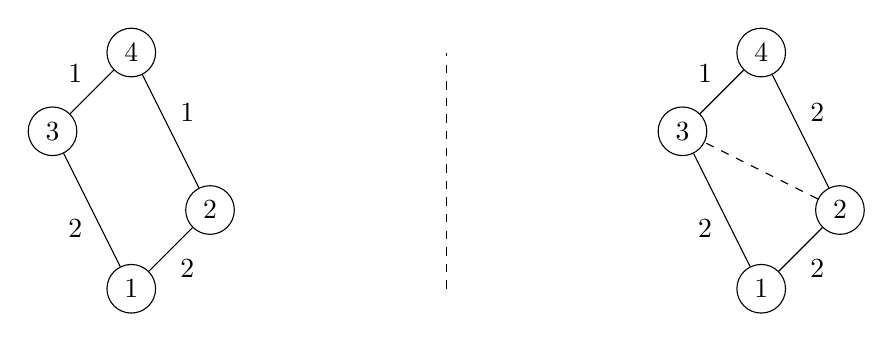
\begin{tikzpicture}[node distance={15mm}, main/.style = {draw, circle}]

    \node[main] (x3) at (0, 2) {$3$};
    \node[main] (x4) at (1, 3) {$4$};
    \node[main] (x2) at (2, 1) {$2$};
    \node[main] (x1) at (1, 0) {$1$};
    
    \draw (x1) -- node[below right] {$2$}(x2);
    \draw (x1) -- node[below left] {$2$} (x3);
    \draw (x2) -- node[above right] {$1$} (x4);
    \draw (x3) -- node[above left] {$1$} (x4);

    \draw[dashed]  (5,0) -- (5,3);

    \node[main] (x31) at (8, 2) {$3$};
    \node[main] (x41) at (9, 3) {$4$};
    \node[main] (x21) at (10, 1) {$2$};
    \node[main] (x11) at (9, 0) {$1$};
    
    \draw (x11) -- node[below right] {$2$}(x21);
    \draw (x11) -- node[below left] {$2$} (x31);
    \draw (x21) -- node[above right] {$2$} (x41);
    \draw (x31) -- node[above left] {$1$} (x41);
    \draw[dashed] (x21) -- node[above, sloped] {}  (x31);

    
\end{tikzpicture}
    \caption{The left represents a CH and the right a CCH contracted graph}
    \label{fig:DifferenceCHAndCCH}
\end{figure}

\subsection{Metric Dependent Vertex Order}
There are two ways to get a suitable vertex order. A so called \textit{metric independent} and a so called \textit{metric dependent} one. The metric independent recursively uses balanced separator to determine a vertex ordering\cite{CCH}. Although this is the superior method, it is not used in this paper writing an algorithm that calculates balanced separators isn't trivial, and we are not aiming for optimizing the contraction process. 
The metric dependent order mainly uses the edge difference $ED$ to determine which vertex is to be contracted next. The $ED$ is determined as the $|edges To Insert| - |edges To Remove|$. The fewer edges are inserted during contraction the fewer edges will be contained by the final graph, therefore fewer edges to expand in a search. However using only the edge differences doesn't lead to desired result. This is because during contraction there will be areas that get less dense than others. 
There are two problems that can arise. One is that important vertices are not contracted last. The other is the search space of the query gets linear although it could be logarithmic.

\subsubsection{Important Vertices not contracted last}\label{sec:not_contracted_last}

\begin{figure}
    \centering
    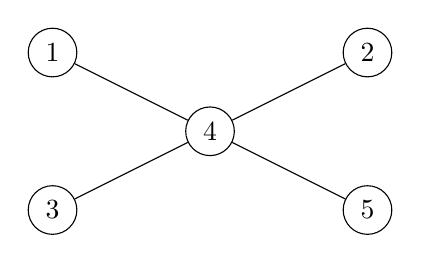
\begin{tikzpicture}[node distance={15mm}, main/.style = {draw, circle}]
    \node[main] (x1) at (1, 2) {$1$}; 
    \node[main] (x3) at (1, 0) {$3$};
    
    \node[main] (x4) at (3, 1) {$4$}; 
    
    \node[main] (x2) at (5, 2) {$2$}; 
    \node[main] (x5) at (5, 0) {$5$}; 
    
    \draw (x1) -- (x4);
    \draw (x2) -- (x4);
    \draw (x3) -- (x4);
    \draw (x5) -- (x4);
    
\end{tikzpicture} 
    
    \caption{The numbers inside the vertices represent their contraction order}
    \label{fig:not_contracted_last}
\end{figure}

Looking at figure \ref{fig:not_contracted_last}, this is a possible contraction order, if only the $ED$ is used to contract vertices. At the beginning the nodes with rank 1, 2, 3, 5 have the same edge difference, which is $ED = -1$. One edge after another will be removed after contraction and the is no shortcut inserted. This happens until there are only the vertices 4 and 5 left. Now vertex 4 has an $ED=-1$, too, same as vertex 5. Therefore the algorithm contracts the vertex with rank 4 before the one with rank 5. \\
However this is not the desired result. There are six ${(1,2), (1,3), (1,5), (2,3), (2,5), (3,5)}$ shortest paths that involve vertex 4, all the other vertices do not encode any shortest path, so vertex 4 should be contracted last. The search graph on the right of Figure \ref{fig:not_contracted_last} shows why. Imagine we we do a shortest path query between $v(1)$ and $v(3)$. After expanding both, the forward and the backward search, to $v(4)$ there is yet another vertex we'll have to expand $v(5)$, although 
as you can see in the original graph on the right, its not possible that $v(5)$ is on the shortest path. Therefore a better contraction order would be a in Figure \ref{fig:contrating_and_searching}.  This can be overcome by the method that is explained in section \ref{sec:vertex_importance}.

\subsubsection{Linear Query Search Space}\label{sec:linear_query}

\begin{figure}
\centering
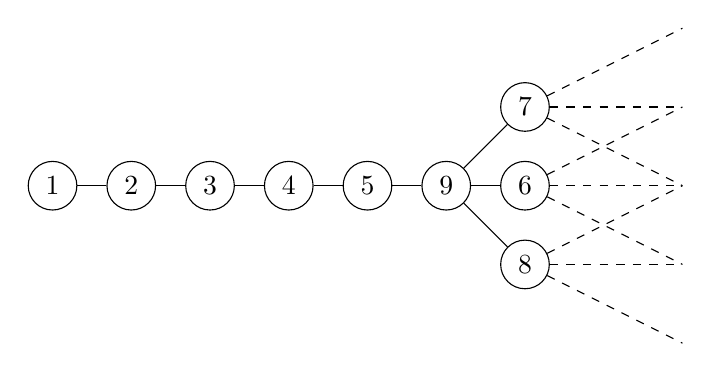
\begin{tikzpicture}[node distance={15mm}, main/.style = {draw, circle}]

    \node[main] (x1) at (0, 0) {$1$};
    \node[main] (x2) at (1, 0) {$2$};
    \node[main] (x3) at (2, 0) {$3$};
    \node[main] (x4) at (3, 0) {$4$};
    \node[main] (x5) at (4, 0) {$5$};
    \node[main] (x9) at (5, 0) {$9$};
    
    \node[main] (x7) at (6, 1) {$7$};
    \node[main] (x8) at (6, -1) {$8$};
    \node[main] (x6) at (6, 0) {$6$};
    
    
    \draw (x1) -- (x2);
    \draw (x2) -- (x3);
    \draw (x3) -- (x4);
    \draw (x4) -- (x5);
    \draw (x5) -- (x9);
    
    \draw (x6) -- (x9);
    \draw (x9) -- (x7);
    \draw (x9) -- (x8);
    
    \draw [dashed] (x7) -- (8, 2);
    \draw [dashed] (x7) -- (8, 1);
    \draw [dashed] (x7) -- (8, 0);
    
    \draw [dashed] (x8) -- (8, 0);
    \draw [dashed] (x8) -- (8, -2);
    \draw [dashed] (x8) -- (8, -1);
    
    \draw [dashed] (x6) -- (8, 1);
    \draw [dashed] (x6) -- (8, 0);
    \draw [dashed] (x6) -- (8, -1);
    
\end{tikzpicture} 
    
\caption{Linear Contraction}
\label{fig:linear_contraction}
\end{figure}

Regarding figure \ref{fig:linear_contraction} there are three possible index graphs $G'$ of one and the same base graph $G$. The numbers inside the vertices represent the contraction order.
\\
The first one could be contracted using the edge difference $ED$, as always one of the outer vertices with $ED=-1$ was contracted. On the one hand it reaches the optimum in case for textit{least shortcuts inserted}. On the other though it has the worst search space among the three vertex orderings. 
To get from node $v(1)$ to $v(5)$ we have to expand four vertices. 
\\
The second $G'$ one contracts the middle vertices, which encodes the most shortest paths, first and therefore inserts three shortcuts. Although this example has a lot of shortcuts, there are still a lot of vertices to expand in some cases. In case every node of $G$ has a weight of $1$, and one wants to go from $v(1)$ to $v(5)$ the forward search will have to expand four nodes as in the upper first example.
\\
The third example contracts the middle node last. At first it contracts the nodes right next to the middle node. Therefore we have to insert shortcuts between $e(v(3)v(5))$ and $e(v(4), v(5))$.
Therefore no matter what source, target pair we are trying to find in this example, the forward and the backward search will have to expand at most one single node. This example additionally shows that
recursively finding a balanced separator, as proposed in \cite[Customization Contraction Hierarchies]{CCH}, is very a promising method to obtain a good contraction order. Sadly there was no time to 
investigate any further in this direction.  

\subsection{Vertex importance}\label{sec:vertex_importance}

As shown in section \ref{sec:not_contracted_last} and \ref{sec:linear_query} using only the $ED$ as a metric to determine which vertex to contract next is not sufficient to get a suitable

\subsection{Perfect Customization}

\begin{figure}
    \centering
    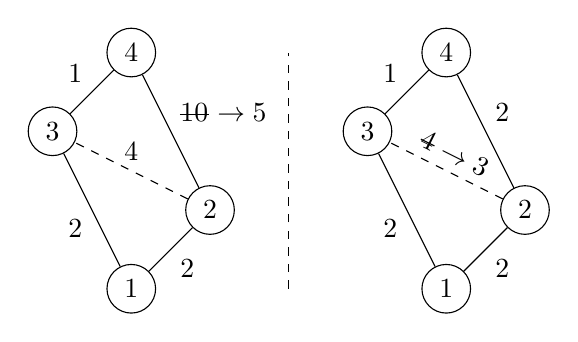
\begin{tikzpicture}[node distance={15mm}, main/.style = {draw, circle}]

    \node[main] (x3) at (0, 2) {$3$};
    \node[main] (x4) at (1, 3) {$4$};
    \node[main] (x2) at (2, 1) {$2$};
    \node[main] (x1) at (1, 0) {$1$};
    
    \draw (x1) -- node[below right] {$2$}(x2);
    \draw (x1) -- node[below left] {$2$} (x3);
    \draw (x2) -- node[above right] {\sout{$10$} $\rightarrow 5$} (x4);
    \draw (x3) -- node[above left] {$1$} (x4);
    \draw[dashed] (x2) -- node[above] {$4$} (x3);

    \draw[dashed]  (3,0) -- (3,3);

    \node[main] (x31) at (4, 2) {$3$};
    \node[main] (x41) at (5, 3) {$4$};
    \node[main] (x21) at (6, 1) {$2$};
    \node[main] (x11) at (5, 0) {$1$};
    
    \draw (x11) -- node[below right] {$2$}(x21);
    \draw (x11) -- node[below left] {$2$} (x31);
    \draw (x21) -- node[above right] {$2$} (x41);
    \draw (x31) -- node[above left] {$1$} (x41);
    \draw[dashed] (x21) -- node[above, sloped] {\sout{$4$} $\rightarrow 3$}  (x31);

    
\end{tikzpicture}
    \caption{Disk Block}
    \label{fig:perfectCustomization}
\end{figure}

Here is an example why perfect customization is necessary to get the full
benefit of CCH.



\chapter{Customizable Contraction Hierarchies}\label{sec:Preliminary_CCH}

In this section we will present the basic idea of \cite[Customization Contraction Hierarchies]{CCH} and also work out the main difference between CCH and \cite[Contraction Hierarchies]{Geisberger_2012}.
It is far form being complete, but there will be some easy examples to show the concept. 

\section{Contracting}

\begin{algorithm}
    \caption{Insert Shortcuts Algorithm}
    \label{alg:contraction}
    \begin{algorithmic}[1]
    \Function{contractGraph}{V}
    \For{$v \in V$} 
        \State queue.offer(getContraction(v))
    \EndFor
    \While{queue is not empty}
    \State $\text{contraction} \gets \text{getContraction(queue.poll())}$
    \State $\text{v} \gets \text{contraction.v}$
    \State $\text{v.rank} \gets \text{rank}$
    \State updateNodeInNeo4J(vertex, rank++)
    \For{$shortcut \in contraction.shortcuts$}
        \State $\text{createOrUpdateEdge}(vertexToContract, shortcut)$
    \EndFor
    \For{$\text{neighbor} \in N_\downarrow(v) \cap N_\uparrow(v)$}
        \State $queue.update(getContraction(neighbor))$
    \EndFor
    \State \Return $v$
    \EndWhile
    \EndFunction

    \Function{getContraction}{v}
    \State$\text{shortcuts} \gets \text{[]}; \text{outerCount, innerCountTimesOuter} \gets 0$
    \For{$\text{inArc} \in \text{v.inArcs}$}
        \If{$\text{inArc.start.rank} = \text{Vertex.UNSET}$}
            \State $\text{outerCount++}; \text{inNode} \gets \text{inArc.start}$
            \For{$\text{outArc} \in \text{v.outArcs}$}
                \If{$\text{outArc.end}.rank = \text{Vertex.UNSET}$}
                    \State $\text{innerCountTimesOuter++; } \text{outNode} \gets \text{outArc.end}$
                    \If{$\text{inNode} \neq \text{outNode}$} $\text{shortcuts.add(Shortcut(inArc, outArc))} $ 
                    \EndIf
                \EndIf
            \EndFor
        \EndIf
    \EndFor
    \State $\text{ED} \gets |shortcuts| - outerCount -  (outerCount \text{ = 0 ? 0 : } \frac{innerCountTimesOuter}{outerCount})$
    \State \Return Contraction(v, ED, shortcuts)
    \EndFunction
    \end{algorithmic}
\end{algorithm}

\begin{figure}
    \centering
    \begin{tikzpicture}[node distance={15mm}, main/.style = {draw, circle}]

    \node[main] (x11) at (0, 0) {$3$};
    \node[main] (x21) at (1, 0) {$1$};
    \node[main] (x31) at (2, 0) {$5$};
    \node[main] (x41) at (3, 0) {$2$};
    \node[main] (x51) at (4, 0) {$4$};
    
    \draw (x11) -- (x21);
    \draw (x21) -- (x31);
    \draw (x31) -- (x41);
    \draw (x41) -- (x51);
    \draw[dashed, out=60, in=120] (x11) to (x31);
    \draw[dashed, out=60, in=120] (x31) to (x51);

    %------------------------------------------------

    \draw[dashed]  (6,0) -- (6,1.5);


    \node[main] (x3) at (8, 0) {$3$};
    \node[main] (x4) at (10, 0) {$4$};
    \node[main] (x5) at (9, 1) {$5$};

    \draw[ -Stealth] (x3) -- (x5);
    \draw[ -Stealth] (x5) -- (x4);
    

\end{tikzpicture}
    \caption{The numbers inside the vertices represent their contraction order}
    \label{fig:contrating_and_searching}
\end{figure}

Algorithm \ref{alg:contraction} provides our contraction algorithm. We do what is called a \textit{metric dependent} contraction in \cite[Customization Contraction Hierarchies]{CCH}. 
This is a greedy algorithm which always takes the next best vertex to contract. Some use the simple edge difference as \cite[Contraction Hierarchies]{Geisberger_2012}, but we will use
a more advanced technique that assigns an importance to each vertex. This importance is further described in section \ref{sec:metric_dependent_importance}, with the equation \ref{eq:importance}.
\\
Before starting we have copied G into G' such that both are identical but refer to their own arc arc vertex set. The input parameter of the \textit{contractGraph} function is the set of vertices V int the input graph G'.
At first we calculate the so called \textit{contraction} for each vertex, which is the set of shortcut arcs that hve to be inserted if that very vertex contracted next. From this contraction object we 
can determine the importance of the vertex. We push the vertex together with its importance into the queue. The  queue is a priority queue that is organized by the importance, such that q. poll will always return the vertex with the 
lowest importance in the queue. As long as the queue is not empty we pull the next vertex and calculate is contraction. We set the rank on the current vertex, initially starts at 0, on the current vertex, add this information to neo4j and increase 
the rank for the next vertex that will be pulled from the queue. 
\\ 
Then we iterate over the shortcut set of the contraction and insert a shortcut into G' where there is yet no arc between vertices. If there is already an arc that connects the vertices of a shortcut, we update the weight of that arc if the shortcut
weight is shorter and update the middle vertex to be able to later on reconstruct the actual path in the input graph G.
Then we iterate ove all neighbors of the just contracted vertex $N_\downarrow(v) \cup N_\uparrow(v)$, recalculate the contraction of these vertices and repush their importance together with the vertex back into the queue. We have to to 
this because the importance of a vertex is dependent on its neighbors. As the neighbors of v just lost a neighbor their importance has to have changed.
After the queue is empty and the algorithm is done, we return top vertex, which is the one with the highest rank. This vertex is later on needed to store the index to the disk.
\\
To get a contraction of a vertex we have to iterate over all connected vertices of v that are not yet contracted. We initialize  a collection of shortcuts to an empty list. Then we iterate over all incoming arcs of v, where the start vertex has not 
yet been contracted. For each of this incoming arc we iterate over all outgoing arcs of which the end vertex has not yet been contracted. Then we create a shortcut container object which is inserted into the shortcut collection. Into the shortcut
we insert the incoming and the outgoing arc.
\\
Finally we calculate the edge difference and insert return the vertex together with the edge difference and the shortcuts.




\subsection{Example}

In Figure \ref{fig:contrating_and_searching} you can see a contracted graph $G'(V,E')$ on the left. The solid lines represent the original edges $E$ of a graph $G$. The dashed lines between vertices are shortcuts $S$ that 
have been added while creating the CCH index graph G'(V, E'). The numbers inside the vertices reflect the contraction order.
\\
Contracting a vertex means deleting it. While contracting a vertex we want to preserve its via connection. If a vertex that is contracted resides on a simple path between two vertices of higher rank,
and there is no edge $e \epsilon E'$ between these vertices a shortcut has to be inserted between the two. 
Let's reconstruct the contraction of Figure \ref{fig:contrating_and_searching}. At first vertex $v(1)$ is removed. As $v(1)$ resides on a simple path to between $v(3)$ and $v(5)$ and there is no edge $e(v(3), v(5)) \notin E'$,
there must be a shortcut added to keep the via path.
The same applies after contracting $v(2)$ for the vertices $v(4)$ and $v(5)$. For all the other vertices we do not need to insert shortcuts.

\section{Searching}

\begin{algorithm}
    \caption{Find Search Path}
    \label{alg:cchSearch}
    \begin{algorithmic}[1]
    \Function{find}{$\text{start}, \text{goal}$}
        \State $\text{pickForward} \gets \text{true};$ $\text{forwardQuery} \gets \text{Query}(\text{start});$$\text{backwardQuery} \gets \text{Query}(\text{goal});$
        \While{not \Call{isComplete}{$\text{forwardQuery, backwardQuery, candidates.peek()}$}}
            \State $\text{query} \gets \text{pickForward} ? \text{forwardQuery} : \text{backwardQuery}$
            \State $\text{other} \gets \text{pickForward} ? \text{backwardQuery} : \text{forwardQuery}$
            \State $\text{pickForward} \gets \neg \text{pickForward}$
            \If{\Call{isNotComplete}{$\text{query}$}}
                 $\text{query.expandNext()}$
            \Else
                 \textbf{ continue}
            \EndIf            
            \State $\text{latest} \gets \text{query.latestExpand()}$
            \If{$\text{other.resultMap().containsKey}(\text{latest.rank})$}
                \State $\text{forwardPath} \gets \text{forwardQuery.getPath}(\text{latest.rank})$
                \State $\text{backwardPath} \gets \text{backwardQuery.getPath}(\text{latest.rank})$
                \State $\text{candidates.offer}(\text{forwardPath} + \text{backwardPath})$
            \EndIf
        \EndWhile
        \State \Return $\text{candidates.poll()}$
    \EndFunction

    \Procedure{expandNext()}{}
    \State $\text{state} \gets \text{queue.poll()}$
    \State $\text{latestExpand} \gets \text{state}$
    
    \If{$\text{goals.contains}(\text{state.getEndVertex().rank}) $}
        \State $\text{shortestPaths.put}(\text{state.getEndVertex().rank}, \text{state.getPath()})$
    \EndIf
    \State $\text{state.settle()}$
    \For{ $\text{arc} \ \text{in} \ \text{state.getEndVertex().arcs}$}
        \State $\text{neighbor} \gets \text{arc.otherVertex}(\text{state.getEndVertex()})$
        \If{\Call{mustUpdateNeighborState}{$\text{state, neighbor, arc.weight}$}}
        \State $\text{newState} \gets \text{state.getPath()} + \text{arc}$
        \State $\text{queue.update}(\text{State}(\text{neighbor, newState}))$
        \State $\text{seen.put}(neighbor.rank, newState)$
            
        \EndIf
    \EndFor
    \EndProcedure
    \end{algorithmic}
\end{algorithm}

Algorithm \ref{alg:cchSearch} shows our search algorithm. It finds the shortest path between the to vertices. As input parameter is takes two integer values, which represent the rank of the start vertex and the rank of the target vertex.
At first init a boolean variable that will us help to choose whether to continue with the forward or with the backward search. Then we initialize one forward query which receives the start vertex as input and all upwards arcs and one backward query that receives 
the target vertex as input and all downward arcs. As long as we have not yet found the certainly we continue the search. We definitely have found the shortest path if either both queries have expanded the top node with the highest rank or 
the next vertex to expand in both queries has a higher weight than the shortest shortest path merge we have seen so far. This is the functionality of \textit{isComplete} function. All shortest path pairs will be merged and pushed to the priority queue that is called \textit{candidates}.
If the search is complete we simply poll and return the next value of the queue which is the shortest path or empty if the vertices are not connected
\\\\
If the search is not complete yet and pick forward is set to \textit{true} we will continue expanding the upward forward query other we will expand die backward query. After that we flip \textit{pickForward}, that at the next iteration set the respective other will be expanded.
If the query we are about expand already reached the top vertex we continue with next iteration step, otherwise we tell the query to expand the next vertex. If the vertex that has be expanded last in the query also appears in the set of already 
expanded vertices in the other query, we merge both their paths and add them to the priority query \textit{candidates} of shortest path pairs found so far. As two merged shortest paths don't necessarily result in a shortest path we still have to continue as described before.



\subsection{Example}

As we preserved all via paths during the contraction the shortest path can be retrieved by a bidirectional Dijkstra that is restricted such that it only expands vertices of higher rank. 
Therefore if one wants to retrieve the shortest path between $v(3)$ and $v(4)$ there will be a forward search from $v(3)$ and a backward search from $v(4)$. As we restrict theses searches to expand only vertices
of higher rank, the only vertices to expand are the start and target vertex. Both will find only one vertex $v(5)$, the highest vertex and the meeting point, too. Finding at least one meeting point in the forward an backward search means there exist a path between them.
After merging these paths at the middle vertex $v(5)$ one will obtain the shortest path.
\\
For an arbitrary contracted graph is it possible that there are more than one meeting point. As merging two shortest paths will not necessary lead to an other shortest path, one has to merge
all possible meeting points and take the path among the merged ones which has the smallest distance. 
\\ 
The stopping condition for such a CH-Search is either, both forward and backward search, have reached the top vertex so there is no further vertex to expand, which happens in the example of figure \ref{fig:contrating_and_searching} or, backward and forward search exceed 
the length that has already been found among the merged paths.


\section{Difference between CH and CCH}

Looking at the left graph in Figure \ref*{fig:DifferenceCHAndCCH} it has been contracted in the CH way, whereas the right is the CCH way. We explicitly state this here because 
we have found paper \cite{Ouyang_2020} that mix up these well known names, claiming they to Contraction Hierarchies CH while actually doing Customizable Contraction Hierarchies CCH. 
The main difference is, CH will only insert an shortcut between two vertices if the vertex that is contracted resides on the shortest path between two of its neighbors. 
When vertex $v(1)$ is contracted there is no shortcut inserted as vertex $v(1)$ is not on the shortest path between which is via vertex $v(4)$.
\\
Whereas in the CCH case the edge weights do not play a role a contraction time. If a vertex is contracted and there is no direct connection between two of its neighbors, one has to insert a shortcut. This gives
the advantage that later on we can easily update edge weights without inserting new shortcut, as all possibly needed shortcuts already exist.
\\ 
Let's complete this example by updating the edge $e(v(2), v(4))$ that currently has the weight of $w(e)=1$ to $w(e) = 5$. Now the vertex $v(1)$ is on the shortest path between vertex $v(2)$ and $v(3)$. 
To update the CH graph we have to insert an edge between vertex $v(2)$ and $v(3)$ whereas the topological structure of the CCH remains the same, one only need to update the weight and the middle vertex of the already give shortcut edge.

\begin{figure}
    \centering
    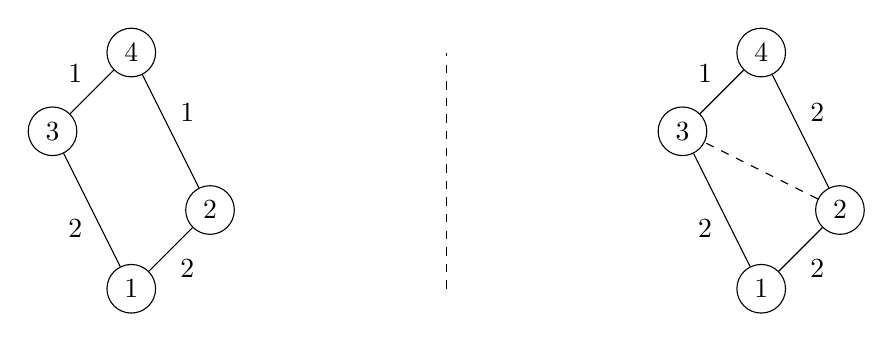
\begin{tikzpicture}[node distance={15mm}, main/.style = {draw, circle}]

    \node[main] (x3) at (0, 2) {$3$};
    \node[main] (x4) at (1, 3) {$4$};
    \node[main] (x2) at (2, 1) {$2$};
    \node[main] (x1) at (1, 0) {$1$};
    
    \draw (x1) -- node[below right] {$2$}(x2);
    \draw (x1) -- node[below left] {$2$} (x3);
    \draw (x2) -- node[above right] {$1$} (x4);
    \draw (x3) -- node[above left] {$1$} (x4);

    \draw[dashed]  (5,0) -- (5,3);

    \node[main] (x31) at (8, 2) {$3$};
    \node[main] (x41) at (9, 3) {$4$};
    \node[main] (x21) at (10, 1) {$2$};
    \node[main] (x11) at (9, 0) {$1$};
    
    \draw (x11) -- node[below right] {$2$}(x21);
    \draw (x11) -- node[below left] {$2$} (x31);
    \draw (x21) -- node[above right] {$2$} (x41);
    \draw (x31) -- node[above left] {$1$} (x41);
    \draw[dashed] (x21) -- node[above, sloped] {}  (x31);

    
\end{tikzpicture}
    \caption{The left represents a CH and the right a CCH contracted graph}
    \label{fig:DifferenceCHAndCCH}
\end{figure}

\section{Metric Dependent Vertex Order}\label{sec:metric_dependent_vertex_order}
There are two ways to get a suitable vertex order. A so called \textit{metric independent} and a so called \textit{metric dependent} one. The metric independent recursively uses balanced separator to determine a vertex ordering\cite{CCH}. Although this is the superior method, it is not used in this paper writing an algorithm that calculates balanced separators isn't trivial, and we are not aiming for optimizing the contraction process. 
The metric dependent order mainly uses the edge difference $ED$ to determine which vertex is to be contracted next. The $ED$ is determined as the $|edges To Insert| - |edges To Remove|$. The fewer edges are inserted during contraction the fewer edges will be contained by the final graph, therefore fewer edges to expand in a search. However using only the edge differences doesn't lead to desired result. This is because during contraction there will be areas that get less dense than others. 
There are two problems that can arise. One is that important vertices are not contracted last. The other is the search space of the query gets linear although it could be logarithmic.

\subsection{Important Vertices not contracted last}\label{sec:not_contracted_last}

\begin{figure}
    \centering
    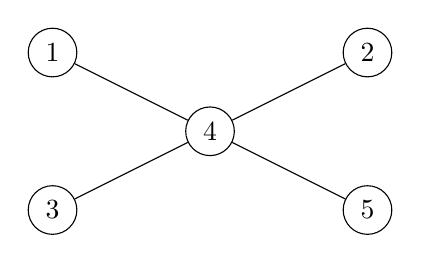
\begin{tikzpicture}[node distance={15mm}, main/.style = {draw, circle}]
    \node[main] (x1) at (1, 2) {$1$}; 
    \node[main] (x3) at (1, 0) {$3$};
    
    \node[main] (x4) at (3, 1) {$4$}; 
    
    \node[main] (x2) at (5, 2) {$2$}; 
    \node[main] (x5) at (5, 0) {$5$}; 
    
    \draw (x1) -- (x4);
    \draw (x2) -- (x4);
    \draw (x3) -- (x4);
    \draw (x5) -- (x4);
    
\end{tikzpicture} 
    
    \caption{The numbers inside the vertices represent their contraction order}
    \label{fig:not_contracted_last}
\end{figure}

Looking at figure \ref{fig:not_contracted_last}, this is a possible contraction order, if only the $ED$ is used to contract vertices. At the beginning the vertices with rank 1, 2, 3, 5 have the same edge difference, which is $ED = -1$. Vertex after vertex is removed  and  no shortcut is inserted. This happens until there are only $v(4)$ and $v(5)$ left. Now $v(4)$ has an $ED=-1$, too, same as vertex 5. Therefore the algorithm contracts $v(4)$ before $v(5)$. However this is not the desired result. There are six \\$e(v(1),v(2)), e(v(1),v(3)), e(v(1),v(5)), e(v(2),v(3)), e(v(2),v(5)), e(v(3),v(5))$  shortest paths that involve  $v(4)$, all the other vertices do not encode any shortest path, so $v(4)$ should be contracted last. The search graph on the right of Figure \ref{fig:not_contracted_last} shows why. Imagine we we do a shortest path query between $v(1)$ and $v(3)$. After expanding both, the forward and the backward search to $v(4)$, there is yet another vertex we'll have to expand $v(5)$. Although 
as you can see in the original graph on the right, its not possible that $v(5)$ is on the shortest path. Therefore a better contraction order would be a in Figure \ref{fig:contrating_and_searching}.  This can be overcome by the method that is explained in section \ref{sec:vertex_importance}.

\subsection{Linear Query Search Space}\label{sec:linear_query}

\begin{figure}
\centering
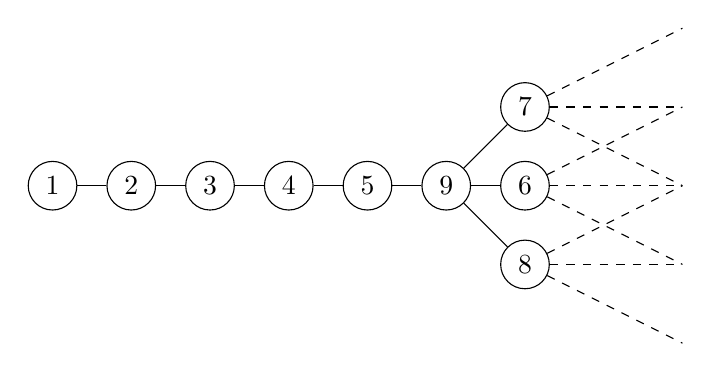
\begin{tikzpicture}[node distance={15mm}, main/.style = {draw, circle}]

    \node[main] (x1) at (0, 0) {$1$};
    \node[main] (x2) at (1, 0) {$2$};
    \node[main] (x3) at (2, 0) {$3$};
    \node[main] (x4) at (3, 0) {$4$};
    \node[main] (x5) at (4, 0) {$5$};
    \node[main] (x9) at (5, 0) {$9$};
    
    \node[main] (x7) at (6, 1) {$7$};
    \node[main] (x8) at (6, -1) {$8$};
    \node[main] (x6) at (6, 0) {$6$};
    
    
    \draw (x1) -- (x2);
    \draw (x2) -- (x3);
    \draw (x3) -- (x4);
    \draw (x4) -- (x5);
    \draw (x5) -- (x9);
    
    \draw (x6) -- (x9);
    \draw (x9) -- (x7);
    \draw (x9) -- (x8);
    
    \draw [dashed] (x7) -- (8, 2);
    \draw [dashed] (x7) -- (8, 1);
    \draw [dashed] (x7) -- (8, 0);
    
    \draw [dashed] (x8) -- (8, 0);
    \draw [dashed] (x8) -- (8, -2);
    \draw [dashed] (x8) -- (8, -1);
    
    \draw [dashed] (x6) -- (8, 1);
    \draw [dashed] (x6) -- (8, 0);
    \draw [dashed] (x6) -- (8, -1);
    
\end{tikzpicture} 
    
\caption{Linear Contraction}
\label{fig:linear_contraction}
\end{figure}

Regarding figure \ref{fig:linear_contraction} there are three possible index graphs $G'$ of one and the same base graph $G$. The numbers inside the vertices represent the contraction order.
\\
The first one could be contracted using the edge difference $ED$, as always one of the outer vertices with $ED=-1$ was contracted. On the one hand it reaches the optimum in case for \textit{least shortcuts inserted}. On the other though it has the worst search space among the three vertex orderings. 
To get from vertex $v(1)$ to $v(5)$ we have to expand four vertices. 
\\
The second $G'$ one contracts the middle vertices, which encodes the most shortest paths, first and therefore inserts three shortcuts. Although this example has a lot of shortcuts, there are still a lot of vertices to expand in some cases. In case every vertex of $G$ has a weight of $1$, and one wants to go from $v(1)$ to $v(5)$ the forward search will have to expand four vertices as in the upper first example.
\\
The third example contracts the middle vertex last. At first it contracts the vertices right next to the middle vertex. Therefore we have to insert shortcuts between $e(v(3)v(5))$ and $e(v(4), v(5))$,
so no matter what source, target pair we are trying to find in this example, the forward and the backward search will have to expand at most one single vertex. This example additionally shows that
recursively finding a balanced separator, as proposed in \cite[Customization Contraction Hierarchies]{CCH}, is very a promising method to obtain a good contraction order. 

\section{Vertex importance}\label{sec:vertex_importance}

As shown in section \ref{sec:not_contracted_last} and \ref{sec:linear_query} there are vertices that are more important that other vertices. Contracting these vertices late is key to get a efficient search later on. 

\subsection{Suitability of CCH}

As it is important to contract important vertices last, the advantage one gets making a CCH search over a simple dijkstra run depends whether the base graph $G(V, E)$ has vertices that are more important than others. 
A vertex $v \epsilon E$ is important if there a many shortest paths that contain this very vertex. Therefore if it is possible to calculate a small balanced separator on $G$, CCH will be able to show its 
whole advantage. To dive deeper into this topic, have a look at \cite[Lower Bounds and Approximation Algorithms for Search Space Sizes in Contraction Hierarchies]{BlumStorandt}.

\subsection{Metric dependent Importance}\label{sec:metric_dependent_importance}

As shown above, taking only the edge difference $ED$ into account doesn't necessarily lead to a proper order, we decided to take the vertex importance calculation that is propose by \cite[Customization Contraction Hierarchies]{CCH}. To every 
vertex we add the level property $l(v)$. The level of the vertex with is initially set to $0$. If a neighbor $w = N(v)$ is contracted level is set to $l(v) = max\{l(v)+1, l(w)\}$. For every arc $a \epsilon A'$
we add a the hop length to the arc $h(a)$. The hop length is equals the number of arcs, this arc represent when fully unpacked. Additionally, we denote as $A(v)$ the set of inserted arcs after the contraction
of $v$ and $D(v)$ the set of removed arcs. We calculate the importance $i(v)$ as follows:

\begin{equation*}
    \label{eq:importance}
    i(v) = l(v) + \frac{|A(v)|}{|D(v)|} + \frac{\sum_{a \epsilon A(v)} h(a)}{\sum_{a \epsilon D(v)} h(a)} 
\end{equation*}

Our tests show that this importance calculation result in slightly increase in the amount of shortcuts added, but the maximum Vertex degree is smaller. Which speeds up the contraction process towards the end. Additionally
the average search time decreases as the search space decreases too. 

% \section{Perfect Customization}
% 
% \begin{figure}
    % \centering
    % 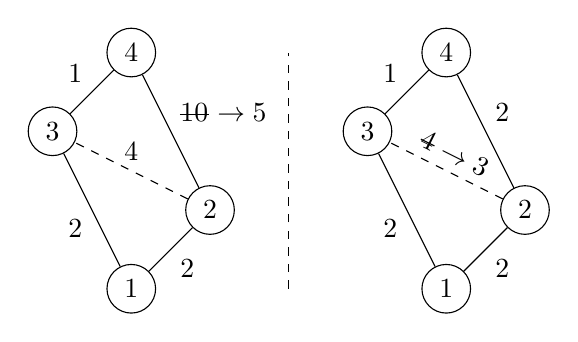
\begin{tikzpicture}[node distance={15mm}, main/.style = {draw, circle}]

    \node[main] (x3) at (0, 2) {$3$};
    \node[main] (x4) at (1, 3) {$4$};
    \node[main] (x2) at (2, 1) {$2$};
    \node[main] (x1) at (1, 0) {$1$};
    
    \draw (x1) -- node[below right] {$2$}(x2);
    \draw (x1) -- node[below left] {$2$} (x3);
    \draw (x2) -- node[above right] {\sout{$10$} $\rightarrow 5$} (x4);
    \draw (x3) -- node[above left] {$1$} (x4);
    \draw[dashed] (x2) -- node[above] {$4$} (x3);

    \draw[dashed]  (3,0) -- (3,3);

    \node[main] (x31) at (4, 2) {$3$};
    \node[main] (x41) at (5, 3) {$4$};
    \node[main] (x21) at (6, 1) {$2$};
    \node[main] (x11) at (5, 0) {$1$};
    
    \draw (x11) -- node[below right] {$2$}(x21);
    \draw (x11) -- node[below left] {$2$} (x31);
    \draw (x21) -- node[above right] {$2$} (x41);
    \draw (x31) -- node[above left] {$1$} (x41);
    \draw[dashed] (x21) -- node[above, sloped] {\sout{$4$} $\rightarrow 3$}  (x31);

    
\end{tikzpicture}
    % \caption{Perfect Customization}
    % \label{fig:perfectCustomization}
% \end{figure}

\section{Update CCH}

\begin{algorithm}
    \caption{Update}
    \begin{algorithmic}[1]
    
    \Procedure{update()}{$G$}
    \State $\text{Q} \gets$ $G'.updatedEdges(G)$; 
    \While{$Q \neq \emptyset $}
        \State $a \gets Q.poll()$; 
        \State $oldWeight \gets w(a)$
        \State $newWeight \gets determineNewWeight(a)$
        \If{$oldWeight != newWeight$}
            \State $w(a) \gets newWeight$
            \State $checkTriangles(Q, oldWeight, upperTriangles(a))$
            \State $checkTriangles(Q, oldWeight, intermediateTriangles(a))$
        \EndIf
    \EndWhile
    \EndProcedure

    \Procedure{checkTriangles}{$Q, oldWeight, triangles$}
    \ForAll{$triangle$ in $triangles$}
        \If{$triangles.c() == triangle.b() + oldWeight$}
            \State{Q.push(triangle.c())}
        \EndIf
    \EndFor
    \State \textbf{return} $\text{triangles}$
    \EndProcedure
        
    \end{algorithmic}
\end{algorithm}

The biggest advantage of CCH over CH is, that it is easy to update without the need of changing the topological structure of the index graph. This is the reason why CCH can be interesting for graph databases.
If an arcs $w(a(x, y))$ weight increases or decreases this can result in a weight change on arcs that connect vertices of higher rank than $x, y$. We determine all arcs of the input graph $G$ that have been changed 
and push them to a priority queue. The queue always pops the the arc $a(x,y)$ with the lowest rank of the start vertex $x$. If there are multiple it pops the one with the lowest rank of $y$ among the ones with the lowest rank of $x$. Then we determine 
the new weight of the arc using the lower triangles. If there is a lower triangle that can be used as a pass through such that the arc weight in $G'$ does not change we do nothing. If the weight of the arc has changed
we assign the new weight to the arc. Then we check all upper triangles, as drawn in figure \ref{fig:updateTriangles}, of $a(x,y)$ if there is an upper arc; denoted by $c$ in figure \ref{fig:updateTriangles}, that is influenced by this very change. If it is influenced by this
change we push it to the priority queue. We do the same with all intermediate triangles. 
\\


\begin{figure}
    \centering
    \begin{tikzpicture}[node distance={15mm}, main/.style = {draw, circle}]

    \node[rotate=90] at (-0.25,0) {rank};
    \draw [ -Stealth]  (0,-2) -- (0,2);

    \node[] at (3,3) {Intermediate Triangles};
    
    \node[main] (z2) at (1, 0) {$z$}; 
    \node[main] (x2) [below right of=z2] {$x$};
    \node[main] (y2) [right of=z2, above of=z2] {$y$}; 
    \draw[ -Stealth] (z2) -- node[above left, sloped] {$c$} (y2);
    \draw[ -Stealth] (z2) -- node[below left, sloped, pos=0.8] {$b$} (x2);
    \draw[ -Stealth] (x2) -- node[below left, sloped] {$a$} (y2);
    \node[] at (2,-2) {$c_\uparrow = a_\uparrow + b_\downarrow $};
    
    \node[main] (z21) at (4, 0) {$z$}; 
    \node[main] (x21) [below right of=z21] {$x$};
    \node[main] (y21) [right of=z21, above of=z21] {$y$}; 
    \draw[ -Stealth] (y21) -- node[above , sloped] {$c$} (z21) ;
    \draw[ -Stealth] (x21) -- node[below right, sloped, pos=0.8] {$b$} (z21);
    \draw[ -Stealth] (y21) -- node[below left, sloped] {$a$} (x21);
    \node[] at (5,-2) {$c_\downarrow = a_\downarrow + b_\uparrow $};

    \node[] at (11,3) {Upper Triangles};
    
    \node[main] (y3) at (9, 0) {$y$}; 
    \node[main] (x3) [below right of=y3] {$x$};
    \node[main] (z3) [right of=y3, above of=y3] {$z$}; 
    \draw[ -Stealth] (z3) -- node[above , sloped] {$c$} (y3);
    \draw[ -Stealth] (x3) -- node[below right, sloped, pos=0.8] {$a$} (y3);
    \draw[ -Stealth] (z3) -- node[below left, sloped] {$b$} (x3);
    \node[] at (10,-2) {$c_\downarrow = a_\uparrow + b_\downarrow$};

    \node[main] (y3) at (12, 0) {$y$}; 
    \node[main] (x3) [below right of=y3] {$x$};
    \node[main] (z3) [right of=y3, above of=y3] {$z$}; 
    \draw[ -Stealth] (y3) -- node[above left, sloped] {$c$} (z3);
    \draw[ -Stealth] (y3) -- node[below left, sloped, pos=0.8] {$a$} (x3);
    \draw[ -Stealth] (x3) -- node[below left, sloped] {$b$} (z3);
    \node[] at (13,-2) {$c_\uparrow = a_\downarrow + b_\uparrow$};

\end{tikzpicture}
    \caption{Update Triangles}
    \label{fig:updateTriangles}
\end{figure}
\chapter{Integration in a Neo4j}

In this section it is described how "Customizable Contraction Hierarchies" CCH is integrated into Neo4j. CCH arguments the input graph, which means it inserts arcs, so called shortcuts, that do not belong to the original data. To keep the change to the input graphs as little as possible we decided to not insert any arc into the graph that is stored inside the neo4j database, but introduce another graph data structure, the index graph. 
The mapping between the index and the graph that resides in the database is achieved by the rank property. The rank property is set to the input and the the index graph at contraction time. Through this we achieve a unique mapping between $G$ and $G'$.
This gives yet another two advantages. One is that we get full control about the graph representation which is helpful to efficiently store and read the index graph for the disk. Another is that with this approach makes it easier to later on port the idea to another graph database manufactures.

\section{Index Graph Data Structure}\label{sec:index_graph}

\begin{figure}
    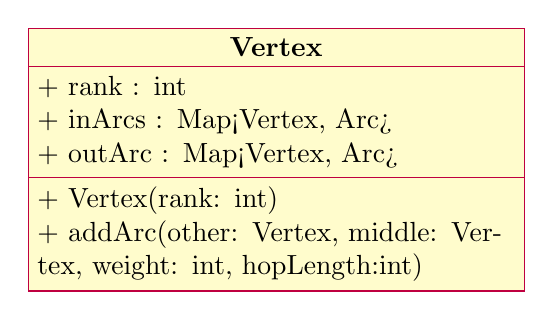
\begin{tikzpicture}
    \begin{class}[text width=0.5\linewidth]{Vertex}{0,0}
        \attribute{+ rank : int}
        \attribute{+ inArcs : Map<Vertex, Arc>}
        \attribute{+ outArc : Map<Vertex, Arc>}
        \operation{+ Vertex(rank: int)}
        \operation{+ addArc(other: Vertex, middle: Vertex, weight: int, hopLength:int) }
      \end{class}
\end{tikzpicture} 
    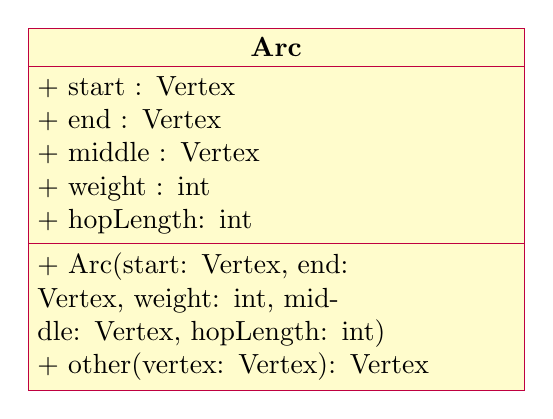
\begin{tikzpicture}
    \begin{class}[text width=0.5\linewidth]{Arc}{0.5\linewidth, 0}
      \attribute{+ start : Vertex}
      \attribute{+ end : Vertex}
      \attribute{+ middle : Vertex}
      \attribute{+ weight : int}
      \attribute{+ hopLength: int}
      \operation{+ Arc(start: Vertex, end: Vertex, weight: int, middle: Vertex, hopLength: int) }
      \operation{+ other(vertex: Vertex): Vertex}
    \end{class}
\end{tikzpicture}
    \caption{Index Graph}
    \label{uml:index_graph}
\end{figure}

The index graph data structure is neither a adjacency list nor adjacency matrix. There is a vertex object that has two hash tables. One for incoming arc and one for outgoing arcs. The hash tables keys are of type vertex and the value is the arc. An arc has a reference to its start vertex and one to its end vertex as shown in figure \ref{uml:index_graph}. 
This also means we cannot construct them all at once, but need a function which initializes the graph, because we have a circular reference. Our solution if you want to initialize such a graph, for an id pair that represents arc or from relationships that come from neo4j is as follows: We iterate over all id pairs, create all vertices that we have not seen so far an push them to a hash table. 
Then create the arc and attach the vertices to it. These vertices we get from the hash table. Finally we add the arc to its start and end vertex.
\\
A disadvantage of this model could be that some modern hardware optimization that exist for arrays do not match with this data structure. Due to paging algorithms as described in \cite[Modern Operatins Systems]{andrew2015modern} when using an array, the values this array are stored sequentially in main memory. When one value of an array is accessed by the CPU, modern hardware reads subsequent values into the CPU-cache because it is likely that they are accessed right after it. The model of the index graph is a linked data structure, a bit like a linked list. The elements of an linked list are contained somewhere in main memory. There is no guarantee that subsequent values have any spacial proximity. Therefore the just explained hardware optimization will not apply. \\ % cite some paper to this topic
However, this makes the the graph traversal easy. Additional it makes it very efficient to explore the neighborhood of a vertex. There is no array traversal to find a vertex and only one hash table lookup for finding an arc of a vertex. Additionally these hash tables only contain few elements. Test on small graphs [Oldenburg] show that cch queries can be answered in less than one millisecond, which is close to what we tested with the original cch application.

\section{The Mapping}\label{sec:mapping}
\begin{figure}
    \centering
    \begin{tikzpicture}[node distance={15mm}, main/.style = {draw, circle}]
 
    \node[main, align=center] (x3) at (0,4) {id:23, labels:\{\\Location,…\}, \\props:\{\\rank:3,…\}};
    \node[main, align=center] (x2) at (12,2) {id:22, labels:\{\\Location,…\}, \\ props:\{\\rank:2,…\}};
    \node[main, align=center] (x1) at (6, 0) {id:21, labels:\{\\Location,…\},  \\ props:\{\\rank:1,…\}};
    
    \draw[ -Stealth] (x2) -- node[rectangle,draw, fill=white,  align=center] {:ROAD \\ weight:1.0}(x1);
    \draw[ -Stealth] (x1) -- node[rectangle,draw, fill=white,  align=center] {:ROAD \\ weight:1.0} (x3);
    \draw[dashed, -Stealth] (x2) -- (x3);

    \draw (0,-2) -- (10,-2);
    \draw (0,-2.5) -- (10,-2.5);
    \draw (0,-3) -- (10,-3);
    \draw (0,-3.5) -- (10,-3.5);
    \draw (0,-4) -- (10,-4);

    \draw (0,-2) -- (0,-4);
    \draw (2.5,-2) -- (2.5,-4);
    \draw (5,-2) -- (5,-4);
    \draw (7.5,-2) -- (7.5,-4);
    \draw (10,-2) -- (10,-4);

    \node[align=center] at (1.25, -2.25) {\textbf{start rank}};
    \node[align=center] at (3.75, -2.25) {\textbf{end rank}};
    \node[align=center] at (6.25, -2.25) {\textbf{middle rank}};
    \node[align=center] at (8.75, -2.25) {\textbf{weight}};

    \node[align=center] at (1.25, -2.75) {2};
    \node[align=center] at (3.75, -2.75) {3};
    \node[align=center] at (6.25, -2.75) {1};
    \node[align=center] at (8.75, -2.75) {2.0};

    \node[align=center] at (1.25, -3.25) {1};
    \node[align=center] at (3.75, -3.25) {3};
    \node[align=center] at (6.25, -3.25) {-1};
    \node[align=center] at (8.75, -3.25) {1.0};

    \node[align=center] at (1.25, -3.75) {2};
    \node[align=center] at (3.75, -3.75) {1};
    \node[align=center] at (6.25, -3.75) {-1};
    \node[align=center] at (8.75, -3.75) {1.0};

\end{tikzpicture}
    \caption{mapping}
    \label{fig:mapping}
\end{figure}

The in memory data structure of neo4j is similar to the just explained index graph data structure in section \ref{sec:index_graph}. A \textit{node} has a collection of \textit{relationships} and a \textit{relationship} has a reference to its \textit{start node} and \textit{end node}.
As neo4j is a full blown property graph nodes and relationship contain a lot of other information. A node has a collection of \textit{labels}, relationship has a \textit{type}. The class \textit{Node} and the class \textit{Relationship} 
are both derived from the class \textit{Entity} which also has a collection of properties as well as and id that is managed by the database system. Note that, as of version Neo4j 5.X, this id can change over time and should not be used to make mappings to external systems. Additionally 
worth to mentioning here is that the Neo4j system shifted its id concept as it moved from major release 4 to 5. Until major release 4 every entity had a unique integer identifier. Since major release 5 every entity has a string identifier which is a UUID and the old \textit{id} identifier
isn't guaranteed to be unique anymore. It is deprecated and marked for removal.
\\
As just explained there are lot of information in this data structure. A lot of information we don't need. Looking at \ref{fig:mapping} we only want to keep track of the information that is needed for the CCH index. Additionally as disks are
divided  into blocks and sectors we want to flatten the graph which is in memory more looks like a tree to a structure that looks like a table. Therefore we decided that the disk data structure only consists of edges $\bigcirc A$. A disk edge $a \epsilon \bigcirc A$ consists of four values, 
the \textit{start rank}, the \textit{end rank}, the \textit{start rank} and the \textit{weight} . The middle node is set $-1$ in case that this arc, is an arc of the input graph. We will get two edge sets $\bigcirc A_\downarrow$ for the downwards graph and $\bigcirc A_\uparrow $ upwards graph.
$\bigcirc A_\downarrow$ contains all downward edge that which are needed for the backward search and $\bigcirc A_\uparrow$ contains all upwards arcs that are needed for the forward search.
\\
During the the contraction every node gets a rank assigned. This rank is the only change that is made to the Neo4j data structure and its the mapping identifier between the input graph $G$ and the index graph $G'$. $G'$ will then be used to generate $\bigcirc A_\downarrow$ and $\bigcirc A_\uparrow$.




\section{How to Store the Index Graph}\label{sec:how_to_store}

\begin{figure}
    \centering
    \begin{tikzpicture}[node distance={15mm}, main/.style = {draw, circle}]
    
    \draw (-7,6) rectangle (-1,7);
    \draw (-5.5,6) -- (-5.5,7);
    \draw (-4,6) -- (-4,7);
    \draw (-2.5,6) -- (-2.5,7);
    \node at (-6.25, 6.5) {from};
    \node at (-4.75, 6.5) {to};
    \node at (-3.25, 6.5) {middle};
    \node at (-1.75, 6.5) {weight};

    \draw [decorate,decoration = {brace, amplitude=5pt}] (-7,7.1) --  (-5.5,7.1);
    \draw [decorate,decoration = {brace, amplitude=5pt}] (-5.5,7.1) --  (-4,7.1);
    \draw [decorate,decoration = {brace, amplitude=5pt}] (-4,7.1) --  (-2.5,7.1);
    \draw [decorate,decoration = {brace, amplitude=5pt}] (-2.5,7.1) --  (-1,7.1);
    \node[ align=center] at (-6.25, 7.8) {32 bit  \\ integer};
    \node[ align=center] at (-4.75, 7.8) {32 bit  \\ integer};
    \node[ align=center] at (-3.25, 7.8) {32 bit  \\ integer};
    \node[ align=center] at (-1.75, 7.8) {32b bit \\ integer};

    \draw [decorate,decoration = {brace, amplitude=5pt}] (-1,5.9) --  (-7, 5.9);
    \node at (-4, 5.5) {16 byte disk arc};

    \draw[dashed, -Stealth] (-1,7) -- (0, 6.7);
    \draw[dashed, -Stealth] (-1,6) -- (0, 6.3);
    
    
    \draw (0,7) -- (4,7);
    \draw[dashed] (0,6) -- (4,6);
    \draw[dashed] (0,5) -- (4,5);
    \node at (4.5,5) {0};
    \node at (4.5,1) {1};
    \draw (0,3) -- (5,3); 
    \draw[dashed] (0,2) -- (4,2);
    \draw[dashed] (0,1) -- (4,1);
    \draw[out=60, in=-120] (0,0) to (4, 0);
    \draw (0,0) -- (0,7); 
    \draw (4,0) -- (4,7); 
    \node at (2, 6.5) {disk arc};
    \node at (2, 5.5) {disk arc};
    \node[rotate=90, font=\Large] at (2, 4) {. . . . .};
    
    \node[rotate=-90] at (5.85, 5) {disk block};
    \draw [decorate,decoration = {brace, amplitude=10pt}] (5.2,7) --  (5.2,3);
\end{tikzpicture}
\caption{Disk Block}
    \label{fig:disk_block}
\end{figure}

After generating the index graph $G'$, we now want to store them as efficiently as possible to the disk. To refine the definition of a disk arc. It consist of four values \textit{start rank}, the \textit{end rank}, the \textit{start rank} and the \textit{weight} as you can see in figure \ref{fig:disk_block}.
\\
This 16 Byte disk arcs are collected to disk blocks. The size of a block can be set as parameter but has two lower bounds. At first a disk block should not be smaller as the block size of the file system beneath as this is the smallest unit once can gets and it would be a wast of space.
The second lower bound is the maximum degree that exists in the index graph after the contraction as all arc of one vertex, as all upward arcs a vertex have to be stored int the same disk block. This applies for the downward arcs, too. 
\begin{equation*}
    max(d_{\uparrow max}(v), d_{\downarrow max}(v)) \leqslant  \frac{diskBlockSize}{16}  
\end{equation*}

\subsection{Persistance Order}\label{sec:persistanceOrder}

\begin{algorithm}
    \caption{DFS in StoreFunction}
    \begin{algorithmic}
        \label{alg:store_dfs}
        \Procedure{store()}{}
        \While{stack $\neq \emptyset$}
            \If{stack.peekFirst().hasNext()}
                \State $\text{vertex} \gets \text{stack.peekFirst().next()}$
                \If{$\lnot$ positionWriter.alreadyWritten(vertex)}
                    \State position $\gets$ arcWriter.write(vertex)
                    \State positionWriter.write(vertex, position)
                    \State stack.addFirst(neighbors(vertex))
                \EndIf
            \Else
                \State stack.pollFirst()
            \EndIf
        \EndWhile
        \EndProcedure      
    \end{algorithmic}
\end{algorithm}


As the disk arcs are later on is used for the CCH search, we want to sequentially write them in a way that provides a high spatial proximity of vertices that are likely to get requested together. Here we will adopt the idea of \cite[Mobile Route Planning]{Sanders}. In the transformation form $G'$ to its disk arcs $\bigcirc A_\uparrow$ 
and $\bigcirc A_\downarrow$ we do a simple depth first search on all ingoing arcs on the target rank to determine the order for $\bigcirc A_\uparrow$. We provided the algorithm for that in algorithm \ref{alg:store_dfs}. As you can see in figure \ref{fig:store_function}, the receives the vertex with the highest rank, whether it shell 
store the upward or the downwards graph and the path, where to store the arcs on the disk. For the upwards graph the mode is set to upwards. At initialization we push an iterator over all incoming vertices that reach the top vertex to stack. Also we open a file write for writing the arc and one file writer for writing the position file as shown in figure \ref{fig:position_file}.
Then we start the \textit{store()} function of algorithm \ref{alg:store_dfs}. As long as the stack is not empty we pick the top iterator of the stack, but leaf it inside. Then we check if that iterator still holds a vertex. If not we remove the iterator and continue. If it holds one we retrieve it. If that vertex hasn't yet been written to the disk,
we tell the arc writer to store it. The arc writer will return the disk block number at which the arcs of that vertex are stored in the arc file. This position writer will keep track of this information. Then we call the neighbors function which get's an iterator of this vertex neighbors sorted ascending by their rank. Finally when the algorithm stops, we write the 
position file to the disk and also flush the rest of the arc file buffer.
\\
We do the same for all the downwards graph using all outgoing instead of the incoming arcs to determine the neighborhood. The arc writer is a write buffer that is as big as the defined disk block size. If during an iteration step there have been more arcs pushed to this arc writer than would fit in the current block, the arc writer flushes 
its cache to the disk, filling the remaining disk arc slots with four times $-1$.

\begin{figure}
    \centering
    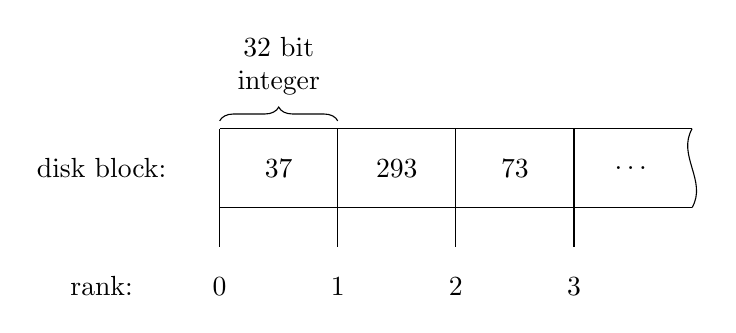
\begin{tikzpicture}[node distance={15mm}, main/.style = {draw, circle}]

    \draw (0,0) -- (6,0);
    \draw (0,1) -- (6,1);
    \draw (0,-0.5) -- (0,1);
    \draw (1.5,-0.5) -- (1.5,1);
    \draw (3,-0.5) -- (3,1);
    \draw (4.5,-0.5) -- (4.5,1);
    \draw[out=60, in=-120] (6,0) to (6,1);

    \node at (0.75, 0.5) {37};
    \node at (2.25, 0.5) {293};
    \node at (3.75, 0.5) {73};
    \node at (5.25, 0.5) {…};

    \node at (-1.5, 0.5) {disk block:};
    \node at (-1.5, -1) {rank:};
    \node at (0, -1) {0};
    \node at (1.5, -1) {1};
    \node at (3, -1) {2};
    \node at (4.5, -1) {3};

    \draw [decorate,decoration = {brace, amplitude=5pt}] (0,1.1) --  (1.5,1.1);
    \node[ align=center] at (0.75, 1.8) {32 bit  \\ integer};

\end{tikzpicture}
    \caption{Position File}
    \label{fig:position_file}
\end{figure}

\begin{figure}
    \centering
    \begin{algorithm}
    \caption{DFS in StoreFunction}
    \begin{algorithmic}
        \label{alg:store_dfs}
        \Procedure{store()}{}
        \While{stack $\neq \emptyset$}
            \If{stack.peekFirst().hasNext()}
                \State $\text{vertex} \gets \text{stack.peekFirst().next()}$
                \If{$\lnot$ positionWriter.alreadyWritten(vertex)}
                    \State position $\gets$ arcWriter.write(vertex)
                    \State positionWriter.write(vertex, position)
                    \State stack.addFirst(neighbors(vertex))
                \EndIf
            \Else
                \State stack.pollFirst()
            \EndIf
        \EndWhile
        \EndProcedure      
    \end{algorithmic}
\end{algorithm}
    \caption{StoreFunction}
    \label{fig:store_function}
\end{figure}

\section{Reading Disk Arcs}

If one wants to get all upwards arcs of rank $i$ one needs take  the upwards position file, retrieve the integer $j$ that is stored at index $i$, and then read the complete block $j$ in the upwards arc file. 
There one will get an array, contain the requested arcs but also some other. These arcs are likely to be request next. Therefore we want to keep them in memory. We implemented two buffer a \textit{circular buffer} and a \textit{least recently used buffer} LRU

\subsection{Circular Buffer}

For the circular buffer we simply used an array of disk arcs. If we reach the end of the buffer we restart overwriting the values from the array start. To get the all arcs of a rank one request that rank number. There is a position hash table which tells the start position of that rank inside the buffer. If it is missing, the containing disk block is read to the buffer. It 
continues to read sequentially until the request rank and the read arc doesn't belong together anymore. This buffer has the advantage that we can exactly determine the amount of arcs we buffering. Also as it is just a simple array, it will be easy for the operation system to cache it.
The disadvantage is that it is possible that we request arc sets very often as it is possible they get evicted just before request again.

\subsection{Least Recently Used Buffer}

Cache is a \textit{java.util.LinkedHashMap}. This class provides the possibility to evicted the entry that has been requested longest time ago. In our case it maps ranks to sets of disk arcs. We can only determine how many 
disk arc sets we have in memory and disk arc sets do not have always the same size. Higher rank vertex usually have bigger sets as they are of higher degree. The advantage is, it is very easy to implement and therefore very 
resilient to programming errors.

\section{The Search}

The search brings all things explained in this chapter together. 

At the beginning there are to index graphs initialized the upwards graph $G_\uparrow'(V_\uparrow, A_\uparrow)$ and the downwards graph $G_\downarrow'(V_\downarrow, A_\downarrow)$. We are looking for the shortest
path from the source vertex $v(s)$ to the target vertex $v(t)$. The vertex set $V_\uparrow$ of the upwards graph $G_\uparrow'(V, A_\uparrow)$ only contains one vertex $v(s)$ and the upward arc set is empty $A_\uparrow = \emptyset$. 
The vertex set $V_\downarrow$ of the downwards graph $G_\downarrow'(V_\downarrow, A_\downarrow)$ only contains the $v(t)$ and the arc set is empty $A_\downarrow = \emptyset$.
Looking at graph in figure \ref{fig:lazy_load_vertex} visualize the search upwards search size after initialization. The ars an vertices in grey are not loaded yet.
\\
As defined earlier in section \ref{sec:dijakstra}, the vertices of the dijkstra query are warped in a object called \textit{DijkstraState} which is define in figure \ref{fig:dijkstra_class}. We now extend this 
class by one parameter, the \textit{VertexLoader} which you can see in figure \ref{fig:lazy_load_vertex}. The \textit{VertexLoader} has only one method \textit{addArcs(vertex: Vertex)}. If you pass a vertex to this method
the VertexLoader will take that vertex and attached all its arcs and their end vertices to it. This happens when the \textit{expandNext()} method in algorithm \ref{alg:disjkstra_algorithm} calls \textit{state.settle()}. This 
follows the observation that the arcs of a vertex in dijkstra are only of interest if the query is about to expand this vertex.
\\
The \textit{VertexManager} get is \textit{DiskArc} from a \textit{Buffer}. The buffer can be of any buffer type it only has to implement \textit{arcs(rank: int):Set<DiskArc>} method. The \textit{VertexManager} is in responsibility 
create the arcs and vertices form the \textit{DiskArc}'s it gets. A \textit{Buffer} contains some type of collection data structure cache \textit{DiskArc}'s. When the vertex manger requests some arcs the \textit{Buffer} checks whether 
they are already cached. If yes it returns them. If not it will request the arcs from the hard drive. This whole process is also visualized in figure \ref{fig:lazy_load_vertex}.
\\
After starting the CH-Dijksta as described in algorithm \ref{alg:cchSearch} both $G_\uparrow'$ and $G_\downarrow'$ are alternatingly expanded and the vertices need will be attached when needed. This can be 
compared to Command \& Conquer or a lot of other strategy  real-time strategy video games where you start at a map that is almost completely grey and the map is only load to the position you are plus some padding.

\begin{figure}
    \centering
    \begin{tikzpicture}[node distance={15mm}, main/.style = {draw, circle}]

    \node[rotate=90] at (-0.25,0) {rank};
    \draw [ -Stealth]  (0,-2) -- (0,2);

    %\node[] at (3,3) {Lower Triangles};
    
    \node[main, draw=black!20] (y) at (1, 0) {$y$}; 
    \node[main] (x) [below right of=y] {$x$};
    \node[main, draw=black!20] (z) [right of=z, above of=y] {$z$}; 

    \draw[ -Stealth, draw=black!20] (x) -- (z);
    \draw[ -Stealth, draw=black!20] (x) -- (y);
    
    \draw[ -Stealth, ] ( 2.5 , -1 ) -- node[above, sloped] {settle()} (5,-0.2);

    \begin{class}[text width=0.2\linewidth]{VertexManager}{7,2}
        \operation{+ VertexManager(b: Buffer)}
        \operation{+ addArcs(vertex: Vertex)}
    \end{class}

    \begin{class}[text width=0.2\linewidth]{Buffer}{14,2}
       \operation{+ arcs(rank: int): Set<DiskArc>}
    \end{class}

    \draw [] (13,-3) -- (13,-2);
    \draw [] (15,-3) -- (15,-2);    

    \draw [out=30, in=-210] (13,-2) to (15,-2);    
    \draw [out=-30, in=-150] (13,-2) to (15,-2);    
    \draw [out=-30, in=-150] (13,-3) to (15,-3); 

    \node[] at (14,-2.7) {Disk};

    \draw [ -Stealth] (13,0) to node[above, sloped] {get(0xFF)} (13,-1.9); 
    \draw [ -Stealth] (15,-1.9) to node[above, sloped] {byte[]} (15,0); 

    \draw [ -Stealth ] (9,2) to node[above, sloped] {arcs(x)} (12,2);    
    \draw [ -Stealth ] (12,0.2) to node[above, sloped] {\{a(x,x), a(x,z)\}} (9,0.2);    


    
\end{tikzpicture}
    \caption{lazy load vertex at query time}
    \label{fig:lazy_load_vertex}
\end{figure}


%\begin{figure}
%    \centering
%    \begin{tikzpicture}[node distance={15mm}, main/.style = {draw, circle}]

    \draw (0,0) -- (9,0);
    \draw (0,1) -- (9,1);
    \draw (0,-0.5) -- (0,1);
    \draw (1.5,-0.5) -- (1.5,1);
    \draw (3,-0.5) -- (3,1);
    \draw (4.5,-0.5) -- (4.5,1);
    \draw (6,-0.5) -- (6,1);
    \draw (7.5,-0.5) -- (7.5,1);
    \draw (9,-0.5) -- (9,1);

    \node<2-4> at (0.75, 0.5) {a(1,x)};
    \node<2-4> at (2.25, 0.5) {a(1,y)};
    \node<2-4> at (3.75, 0.5) {a(1,z)};
    \node<5-> at (0.75, 0.5) {a(3,x)};
    \node<5-> at (2.25, 0.5) {a(3,y)};
    \node<5-> at (3.75, 0.5) {a(3,z)};
    \node<3-4> at (5.25, 0.5) {a(2,x)};
    \node<5-> at (5.25, 0.5) {a(3,zx)};
    \node<3-> at (6.75, 0.5) {a(2,y)};
    \node<3-> at (8.25, 0.5) {a(2,z)};

    \node at (-1.5, 0.5) {DiskArc[]};
    \node at (-1.5, -1) {index:};
    \node at (0, -1) {0};
    \node at (1.5, -1) {1};
    \node at (3, -1) {2};
    \node at (4.5, -1) {3};
    \node at (6, -1) {4};
    \node at (7.5, -1) {5};
    \node at (9, -1) {size};

    \draw<1>[ -Stealth, ] (0, -4 ) -- node[above, sloped] {writePointer} (0,-1.5);
    \draw<2>[ -Stealth, ] (4.5, -4 ) -- node[above, sloped] {writePointer} (4.5,-1.5);
    \draw<3-4>[ -Stealth, ] (0, -4 ) -- node[above, sloped] {writePointer} (0,-1.5);
    \draw<5-6>[ -Stealth, ] (6, -4 ) -- node[above, sloped] {writePointer} (6,-1.5);



    \node at (-1.5, 2) {positions:};
    \onslide<1>{\node (tab1)  at (3,2) {%
        \begin{tabular}{c }
            \textbf{rank} \\
            \hline
            \textbf{position} \\
        \end{tabular}};
    }
    \onslide<2>{\node (tab1)  at (3,2) {%
        \begin{tabular}{c | c }
            \textbf{rank} & 1  \\
            \hline
            \textbf{position} & 2  \\
        \end{tabular}};
    }
    \onslide<3>{\node (tab1)  at (3,2) {%
        \begin{tabular}{c | c | c }
            \textbf{rank} & 1 & 2 \\
            \hline
            \textbf{position} & 2 & 5 \\
        \end{tabular}};
    }
    \onslide<4>{\node (tab1)  at (3,2) {%
        \begin{tabular}{c | c | c | c}
            \textbf{rank} & 1 & 2 & max(rank) \\
            \hline
            \textbf{position} & 2 & 5 & -1 \\
        \end{tabular}};
    }
    \onslide<5>{\node (tab1)  at (3,2) {%
        \begin{tabular}{c | c | c | c | c}
            \textbf{rank} & 1 & \textcolor{red}{2} & 3 & max(rank) \\
            \hline
            \textbf{position} & 2 & \textcolor{red}{5} & 3 & -1 \\
        \end{tabular}};
    }
    \onslide<6->{\node (tab1)  at (3,2) {%
        \begin{tabular}{c | c | c | c }
            \textbf{rank} & 1 & 3 & max(rank) \\
            \hline
            \textbf{position} & 2 & 3 & -1 \\
        \end{tabular}};
    }

    \onslide<5>{
      \node at (0,-2){\textcolor{red}{remove incomplete edge set from position}};
    }
   

\end{tikzpicture}
%    \caption{Circular Buffer}
%    \label{fig:circular_buffer}
%\end{figure}

\chapter{Experiments}

In this chapter we will experimentally check if our idea and implementation of a persisted version of CCH works out.

\section{The Test Environment}

We implemented this CCH in \textit{Java 17} and fo \textit{Neo4j 5.1.0}. The only addition Java library we use is \textit{lombok version 1.18.24}, for static code generation, like getter and setters.
\\
The code runs on a virtual machine that is running \textit{Linux Mint 20.3 Una}. This VM has two  AMD EPYC 7351 16-Core Processors with L1d cache=1 MiB L1i cache=2 MB, L2 cache=16 MB and L3 cache=128 MB. 
It has 512 GB of RAM and the system hard drive is a \textit{Intel SSDPEKNW020T8} SSD with 2 TB.


\section{The Test Data}

The test graphs we evaluate the implementation are provided by the \cite[9th DIMACS Implementation Challenge - Shortest Paths]{DIMACS}. There we focus on the road networks of New York, Colorado, Florida and California+Nevada.
We use the distance graphs, only in case of New York we tried the distance and the time travel graph. As the results were similar and the contraction strategy is not depending on the arc weight we omitted the further test wit the time travel graphs.

\section{The Contraction}

In table \ref{tab:overview_table} you can see the basic results of the networks we tested. One would think that the contraction time goes along with the size of the network, though it doesn't. The New York graph has has about the same contraction time 
as Florida which is about three times as big. Additionally the amount of shortcuts inserted Relative to the already existing arcs is almost twice as big. This is probably happens because the New York graph is a lot denser than the other graphs under test like Florida.
In New York, regardless if you take the state or only the city itself, there are four natural separators: \textit{Manhattan and Brooklyn}, \textit{Manhattan and Queens}, \textit{Manhattan and Bronx}, \textit{Bronx and Queens}, \textit{Staten Island and Brooklyn} as well as \textit{Staten Island and Manhattan to the mainland}.  
\\ 
Where as the population of Florida is more sparse and located on a line at the cost of both side, as well as their streets. Therefore as shown in figure \ref{fig:linear_contraction} the contraction can easily find vertices as separators. 

\subsection{Limits}

We decided to set the time limit a contraction should not exceed to one day. If, within this time the contraction did finish, we decided to abort the process. This happend for the graphs \textit{Western USA, …}. If one would want to go this size or bigger we suggest,
to achieve the vertex ordering by recursive finding balanced separators as described in \cite[Customization Contraction Hierarchies]{CCH}. 
\\
Contraction methods that rely on measures like edge difference suffer from very bad performance, if the graph gets dense. At the same time, the remaining graph will get denser towards the end of the contraction process. It is possible  that the last few nodes form a complete graph. The algorithm
as proposed in this paper always will update the importance  of it's neighbors  after each contracted vertex and re-push it to the queue $Q$ of remaining vertices. Update the neighbor importance means to simulate the contraction of this neighbor. So we check for all pairs of incoming and outgoing neighbors $N_\downarrow(v) \times N_\uparrow(v) \setminus N_\downarrow(v) = N_\uparrow(v)$ whether we have to insert a shortcut. 
This you have to $|Q|$ times. In case of a complete graph the in- and the outgoing neighbor set will have size $|Q|$. Which lead to the this many neighbor checks $(|Q| * |Q| - |Q|)*|Q|$ which is almost $(|Q|)^3$ checks whether to insert a shortcut or not. In case your graph already get's complete or close to it on the last 
100 this is a doable exercise. In case there are 3000 remaining, it will starve. 


\begin{table}
    \centering
    \begin{tabular}{ p{5cm} || R{2cm} | R{2cm} | R{2cm} | R{2cm} }
    \toprule
     & \multicolumn{1}{l}{\textbf{New York}} & \multicolumn{1}{l}{\textbf{Colorado}} & \multicolumn{1}{l}{\textbf{Florida}} & \multicolumn{1}{L{2cm}}{\textbf{California + Nevada}} \\ 
    \midrule
    Verticies & 264,346 & 435,666 & 1,070,376 & 1,890,815 \\
    Edges & 733,846 & 1,057,066 & 2,712,798 & 4,657,742 \\
    Shortcuts & 2,153,002 & 1,680,290 & 4,397,804 & 8,598,552 \\
    Shortcuts added Relative & 2.93 & 1.59 & 1.62 & 1.85 \\
    Contraction Time & 545 s & 233 s & 579 s & 4,384 s \\
    Max In Degree & 1,150 & 629 & 785 & 1,252 \\
    Out Arcs Disk Size & 23.1 MB & 21.9 MB & 56.9 MB & 106.5 MB \\ 
    Out Position File Size & 1.1 MB & 1.8MB & 1.3MB & 7.6 MB \\ 
    In Arcs Disk Size & 23.1 MB & 21.9 MB & 56.9 MB & 106.5 MB \\ 
    In Position File Size & 1.1 MB & 1.8MB & 1.3MB & 7.6 MB \\ 
    Block filling & 0.99 & 0.95 & -122.0 & -122.0 \\ 
    AVG Dijkstra Search Time & 0.816 s & 0.549 s & 2.630 s & 4.858 s \\ 
    AVG Search Time (40kB) & 0.140 s & 0.122 s & 0.147 s & 0.289 s\\
    AVG Disk Access (40kB) & 574 & 437 & 500 & 899 \\
    Update Time & 90 s & 51 s & 142 s & 444 s \\
    AVG Search Time (40kB) after multi update & 0.147 s & 0.129 s & 0.150 s & 0.302 \\
    AVG Disk Access (40kB) after multi update & 569 & 457 & 516 & 924 \\
    \bottomrule
    \end{tabular}
    \caption{Network overview table}
    \label{tab:overview_table}
\end{table}


\section{Query Performance}

In this section we will have a look at the query performance. The query performance will depends mainly in quality of the contraction and the buffer size. 
As the circular buffer we implemented performs better we will focus on it and bring only a small comparison at the end to the LRU buffer.


\subsection{Comparison with Dijkstra}

Regarding Figure \ref{fig:dijkstra_vs_cch_query_speed} shows speed difference of Dijkstra and CCH-shortest path query. As you can see, the greater distance, the greater the advantage of CCH over dijkstra. Small queries where the shortest path involve only a few hundred vertices have a very little speed up,
whereas long distance queries are a lot faster. Figure \ref{fig:dijkstra_vs_cch_query_speed} is a random sample of queries in California and Nevada. As you can
see in the left chart, there are some long distance queries for which dijkstra performs very good, though you cannot see them in the right chart, that has the path 
length on the x-axis. We assume the good performing long distance queries to be in Nevada as its road network is sparser and than those of California. Therefore we added the right chart.
It shows the advantage of CCH over dijkstra depends on the path length of the shortest path.


\begin{figure}   
\begin{tikzpicture}
    \begin{axis}[
        title={Query Time over Distance},
        xlabel={distance},
        ylabel={time in micro seconds},
        legend pos=north west,
        xmajorgrids=true,
        ymajorgrids=true,
        grid style=dashed,
        width = 0.54\linewidth,
    ]
        
        \addplot table [x=weight, y=dijkstraTime, col sep=comma, only marks] {assets/plots/cal-data.csv};
        \legend{dijkstra, CCH}
        \addplot table [x=weight, y=cchTime, col sep=comma, only marks] {assets/plots/cal-data.csv};
    \end{axis}
\end{tikzpicture}
\begin{tikzpicture}
    \begin{axis}[
        title={Query Time over Path length},
        xlabel={dijkstra path length},
        %ylabel={time in micro seconds},
        legend pos=north west,
        xmajorgrids=true,
        ymajorgrids=true,
        grid style=dashed,
        width = 0.54\linewidth
    ]
        
        \addplot table [x=dijkstraHops, y=dijkstraTime, col sep=comma, only marks] {assets/plots/cal-data.csv};
        \legend{dijkstra, CCH}
        \addplot table [x=dijkstraHops, y=cchTime, col sep=comma, only marks] {assets/plots/cal-data.csv};
    \end{axis}
\end{tikzpicture}
\caption{Comparison of CCH query performance on the California+Nevada graph, before updating. Buffer size 40kB. Random sample of 1000 vertex to vertex queries}
\label{fig:dijkstra_vs_cch_query_speed}
\end{figure}

Having a look a figure \ref{fig:dijkstra_vs_cch_expanded_vertices} we compare the amount of vertices the search query has to expand to find the shortest path. As expected dijkstra expands roughly quadratic many vertices to find the shortest path between vertices for shortest paths that involve up to 1000 vertices.
After that the search touches the network borders and starts to expand the last leaves which happens almost linear.\\
The CCH search only expands vertices of higher rank. As you can see in Figure \ref{fig:dijkstra_vs_cch_expanded_vertices} the CCH expands at most around 1600 vertices. Therefore, we assume, CCH needs at most expand 800 vertices per search side the find the node with the highest rank. So no matter which source or target one chooses, the query will be bound to these 1600 vertex expansions.
This is the reason CHH performs so good especially for long distance queries.
\\
So far we only had a look long distance queries, let's have a look at the short ones, but queries where source and target are more that 300 vertices away already perform as good or better than dijkstra. The search sides of these queries are even shorter than 800 expanded vertices. They can figure out the shortest path within a few hundred node expansions.

\begin{figure}   
    \begin{tikzpicture}
        \begin{axis}[
            title={Query Time over Distance},
            xlabel={distance},
            ylabel={Expanded Nodes},
            legend pos=north west,
            xmajorgrids=true,
            ymajorgrids=true,
            grid style=dashed,
            width = 0.54\linewidth,
        ]
            
            \addplot table [x=dijkstraHops, y=DijkstraExpandedNodes, col sep=comma, only marks] {assets/plots/data.csv};
        \end{axis}
    \end{tikzpicture}
    \begin{tikzpicture}
        \begin{axis}[
            title={Query Time over Path length},
            xlabel={dijkstra path length},
            %ylabel={time in micro seconds},
            legend pos=north west,
            xmajorgrids=true,
            ymajorgrids=true,
            grid style=dashed,
            width = 0.54\linewidth
        ]
            
        \addplot table [x=dijkstraHops, y=cchExpanded, col sep=comma, only marks] {assets/plots/data.csv};
         \end{axis}
    \end{tikzpicture}
    \caption{Comparison of CCH query performance on the California+Nevada graph, before updating. Buffer size 40kB. Random sample of 1000 vertex to vertex queries}
    \label{fig:dijkstra_vs_cch_expanded_vertices}
\end{figure}

\subsection{Disk Access at Query Time}

some text


\begin{tikzpicture}
    \begin{axis}[
        title={Disk access over Expand Nodes in CCH},
        xlabel={Expanded Verticies},
        ylabel={Load Invocations},
        legend pos=north west,
        xmajorgrids=true,
        ymajorgrids=true,
        grid style=dashed,
        width = 1\linewidth
    ]
    \addplot table [x=cchExpanded, y=cchLoadInvocations, col sep=comma, only marks] {assets/plots/data.csv};
    \end{axis}
\end{tikzpicture}

\begin{tikzpicture}
    \begin{axis}[
        title={Disk access over Time in CCH},
        xlabel={Time},
        ylabel={Load Invocations},
        legend pos=north west,
        xmajorgrids=true,
        ymajorgrids=true,
        grid style=dashed,
        width = 1\linewidth
    ]
    \addplot table [x=cchTime, y=cchLoadInvocations, col sep=comma, only marks] {assets/plots/data.csv};
    \end{axis}
\end{tikzpicture}

\begin{tikzpicture}
    \begin{axis}[
        title={Disk access over Expand Nodes in CCH},
        xlabel={Dijkstra path length},
        ylabel={CCH path length},
        legend pos=north west,
        xmajorgrids=true,
        ymajorgrids=true,
        grid style=dashed,
        width = 1\linewidth,
        %x filter/.code={\pgfmathparse{#1^0.5}}
        %xmode = log,
        %log basis x=2
        ]
    \addplot table [x=dijkstraHops, y=cchHops, col sep=comma, only marks] {assets/plots/data.csv};
    \end{axis}
\end{tikzpicture}

\begin{tikzpicture}
    \begin{axis}[
        title={Disk access over Expand Nodes in CCH},
        xlabel={Path Length},
        ylabel={Distance},
        legend pos=north west,
        xmajorgrids=true,
        ymajorgrids=true,
        grid style=dashed,
        width = 1\linewidth
    ]
    \addplot table [x=weight, y=cchHops, col sep=comma, only marks] {assets/plots/data.csv};
    \addplot table [x=weight, y=dijkstraHops, col sep=comma, only marks] {assets/plots/data.csv};
    \legend{dijkstra, CCH}
    \end{axis}
\end{tikzpicture}

\begin{tikzpicture}
    \begin{axis}[
        title={Expanded Verticies over Path Length},
        xlabel={Distance},
        ylabel={Expanded Verticies},
        legend pos=north west,
        xmajorgrids=true,
        ymajorgrids=true,
        grid style=dashed,
        width = 1\linewidth
    ]
    \addplot table [x=weight, y=DijkstraExpandedNodes, col sep=comma, only marks] {assets/plots/data.csv};
    \addplot table [x=weight, y=cchExpanded, col sep=comma, only marks] {assets/plots/data.csv};
    \legend{dijkstra, CCH}
    \end{axis}
\end{tikzpicture}

\begin{tikzpicture}
    \begin{axis}[
        title={Expanded Verticies over Distance},
        xlabel={Path Length},
        ylabel={Expanded Verticies},
        legend pos=north west,
        xmajorgrids=true,
        ymajorgrids=true,
        grid style=dashed,
        width = 1\linewidth
    ]
    \addplot table [x=dijkstraHops, y=DijkstraExpandedNodes, col sep=comma, only marks] {assets/plots/data.csv};
    \addplot table [x=dijkstraHops, y=cchExpanded, col sep=comma, only marks] {assets/plots/data.csv};
    \legend{dijkstra, CCH}
    \end{axis}
\end{tikzpicture}

\newpage


\chapter{Future Work}

With this work we barely scratched the surface of what can be done with CCH in neo4j. 
There are a lot of special topics one could dive deeper to improve CCH for neo4j.

\section{Contraction Algorithms}

As the contraction algorithm \ref{alg:contraction} we use definitely has its limitation as we have seen in the experiment section \ref{sec:contraction_limits}, it is worth digging
deeper there. One very promising method determine the vertex by recursively look for minimum balanced separators until they tend to get big and then continue with our algorithm.
Another question we haven't even touched is, what if we add vertices and arcs. How can we deal with such updates in the input graph which are not unusual for databases.

\section{The Test Dataset}

Changing the test domain can be interesting, too. Most papers like \cite[CCH]{CCH}, and \cite[CH]{Geisberger_2012} and many more focus on road networks. This definitely made sense for this
paper to also check if we come to similar results. However, one could also try grids as \cite[Storandt]{storandt2013contraction} or looking for other real world domains that can be modeled such that shortest path queries are of major interest.

\section{Perfect Customization and Transition to CH}

\begin{wrapfigure}{r}{0.5\textwidth}
    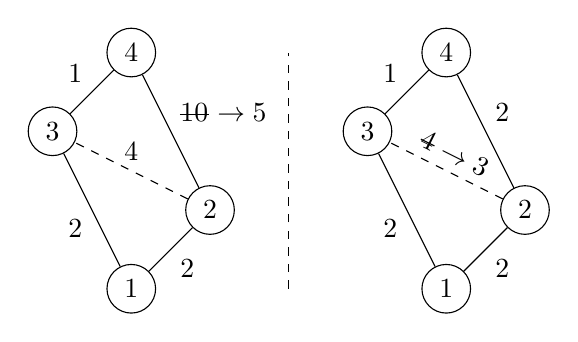
\begin{tikzpicture}[node distance={15mm}, main/.style = {draw, circle}]

    \node[main] (x3) at (0, 2) {$3$};
    \node[main] (x4) at (1, 3) {$4$};
    \node[main] (x2) at (2, 1) {$2$};
    \node[main] (x1) at (1, 0) {$1$};
    
    \draw (x1) -- node[below right] {$2$}(x2);
    \draw (x1) -- node[below left] {$2$} (x3);
    \draw (x2) -- node[above right] {\sout{$10$} $\rightarrow 5$} (x4);
    \draw (x3) -- node[above left] {$1$} (x4);
    \draw[dashed] (x2) -- node[above] {$4$} (x3);

    \draw[dashed]  (3,0) -- (3,3);

    \node[main] (x31) at (4, 2) {$3$};
    \node[main] (x41) at (5, 3) {$4$};
    \node[main] (x21) at (6, 1) {$2$};
    \node[main] (x11) at (5, 0) {$1$};
    
    \draw (x11) -- node[below right] {$2$}(x21);
    \draw (x11) -- node[below left] {$2$} (x31);
    \draw (x21) -- node[above right] {$2$} (x41);
    \draw (x31) -- node[above left] {$1$} (x41);
    \draw[dashed] (x21) -- node[above, sloped] {\sout{$4$} $\rightarrow 3$}  (x31);

    
\end{tikzpicture}
    
\end{wrapfigure}

We didn't implement the perfect customization, nor the transition from CCH to CH. A CH index is usually faster at query time as the amount of arcs is less. Therefore it can be useful to have 
a CCH and always calculate a CH from it after each update. In that scenario it is also useful to measure how long such a transition takes.

\section{Using relational Databases}

Furthermore it is questionable if graph databases like neo4J solve any problem. Due to \cite[The Case Against Specialized Graph Analytics Engines]{fan2015case} there is no significant difference in processing a graph in a graph database compared to a relational 
database. Therefore it would be interesting to see, how an implementation of dijkstra and (C)CH perform in SQL, written for relational databases. 
\begin{frame}
    \frametitle{Conclusion}
    
    \begin{itemize}
        \item We can accelerate Graph Databases with CCH
        \item The major problem is to flatten the graph
        \item Try it with a Relational Database
    \end{itemize}

\end{frame}

\bibliography{related.bib}
\addcontentsline{toc}{chapter}{Bibliography}


\end{document}
